\documentclass[12pt]{article}

%==============Packages & Commands==============
\usepackage{graphicx}
\usepackage{fancyvrb}
\usepackage{array}
\usepackage{tikz}
%%%<
\usepackage{listings}
%\usepackage[active,tightpage]{preview}
%\PreviewEnvironment{tikzpicture}
%\setlength\PreviewBorder{5pt}%

\usepackage{geometry}                		% See geometry.pdf to learn the layout options. There are lots.
\geometry{letterpaper}                   		% ... or a4paper or a5paper or ...
%\geometry{landscape}                		% Activat\usetikzlibrary{arrows}e for for rotated page geometry
%\usepackage[parfill]{parskip}    		% Activate to begin paragraphs with an empty line rather than an indent
\usepackage{graphicx}				% Use pdf, png, jpg, or eps§ with pdflatex; use epFs in DVI mode
								% TeX will automatically convert eps --> pdf in pdflatex
\usepackage{amsmath}
\usepackage{amssymb}

%\usepackage[ruled,vlined]{algorithm2e}
\usetikzlibrary{arrows}
\usepackage{alltt}
\usepackage[T1]{fontenc}
%\usepackage[utf8]{inputenc}
\usepackage{indentfirst}
\usepackage[longnamesfirst]{natbib} % For references
\bibpunct{(}{)}{;}{a}{}{,} % Reference punctuation
\usepackage{changepage}
\usepackage{setspace}
\usepackage{booktabs} % For tables
\usepackage{floatrow}
\usepackage{rotating} % For sideways tables/figures
\usepackage{amsmath}
\usepackage{multirow}
\usepackage{color}
 
\definecolor{codegreen}{rgb}{0,0.6,0}
\definecolor{codegray}{rgb}{0.5,0.5,0.5}
\definecolor{codepurple}{rgb}{0.58,0,0.82}
\definecolor{backcolour}{rgb}{0.95,0.95,0.92}
 
\lstdefinestyle{mystyle}{
    backgroundcolor=\color{backcolour},   
    commentstyle=\color{codegreen},
    keywordstyle=\color{magenta},
    numberstyle=\tiny\color{codegray},
    stringstyle=\color{codepurple},
    basicstyle=\footnotesize,
    breakatwhitespace=false,         
    breaklines=true,                 
    captionpos=b,                    
    keepspaces=true,                 
    numbers=left,                    
    numbersep=5pt,                  
    showspaces=false,                
    showstringspaces=false,
    showtabs=false,                  
    tabsize=2
}
 
\lstset{style=mystyle}
\usepackage{dcolumn}
\usepackage{comment}
%\usepackage{fullwidth}
\newcolumntype{d}[1]{D{.}{\cdot}{#1}}
\newcolumntype{.}{D{.}{.}{-1}}
\newcolumntype{3}{D{.}{.}{3}}
\newcolumntype{4}{D{.}{.}{4}}
\newcolumntype{5}{D{.}{.}{5}}
\usepackage{float}
\usepackage[hyphens]{url}
%\usepackage[margin = 1.25in]{geometry}
%\usepackage[nolists,figuresfirst]{endfloat} % Figures and tables at the end
\usepackage{subfig}
\captionsetup[subfloat]{position = top, font = normalsize} % For sub-figure captions
\usepackage{fancyhdr}
%\makeatletter
%\def\url@leostyle{%
%  \@ifundefined{selectfont}{\def\UrlFont{\sf}}{\def\UrlFont{\small\ttfamily}}}
%\makeatother
%% Now actually use the newly defined style.
\urlstyle{same}
\usepackage{times}
\usepackage{mathptmx}
%\usepackage[colorlinks = true,
%						bookmarksopen = true,
%						pagebackref = true,
%						linkcolor = black,
%						citecolor = black,
% 					urlcolor = black]{hyperref}
%\usepackage[all]{hypcap}
%\urlstyle{same}
\newcommand{\fnote}[1]{\footnote{\normalsize{#1}}} % 12 pt, double spaced footnotes
\def\citeapos#1{\citeauthor{#1}'s (\citeyear{#1})}
\def\citeaposs#1{\citeauthor{#1}' (\citeyear{#1})}
\newcommand{\bm}[1]{\boldsymbol{#1}} %makes bold math symbols easier
\newcommand{\R}{\textsf{R}\space} %R in textsf font
\newcommand{\netinf}{\texttt{NetInf}\space} %R in textsf font
\newcommand{\iid}{i.i.d} %shorthand for iid
\newcommand{\cites}{{\bf \textcolor{red}{CITES}}} %shorthand for iid
%\usepackage[compact]{titlesec}
%\titlespacing{\section}{0pt}{*0}{*0}
%\titlespacing{\subsection}{0pt}{*0}{*0}
%\titlespacing{\subsubsection}{0pt}{*0}{*0}
%\setlength{\parskip}{0pt}
%\setlength{\parsep}{0pt}
%\setlength{\bibsep}{2pt}
%\renewcommand{\headrulewidth}{0pt}

%\renewcommand{\figureplace}{ % This places [Insert Table X here] and [Insert Figure Y here] in the text
%\begin{center}
%[Insert \figurename~\thepostfig\ here]
%\end{center}}
%\renewcommand{\tableplace}{%
%\begin{center}
%[Insert \tablename~\theposttbl\ here]
%\end{center}}

\newcommand\independent{\protect\mathpalette{\protect\independenT}{\perp}}
\def\independenT#1#2{\mathrel{\rlap{$#1#2$}\mkern2mu{#1#2}}}
\newcommand{\N}{\mathcal{N}}
\newcommand{\Y}{\bm{\mathcal{Y}}}
\newcommand{\bZ}{\bm{Z}}

\usepackage[colorlinks = TRUE, urlcolor = black, linkcolor = black, citecolor = black, pdfstartview = FitV]{hyperref}


%============Article Title, Authors==================
\title{\vspace{-2cm} Considering Network Effects in the Design and Analysis of Field Experiments on State Legislatures } 


%\author{Sayali Phadke \thanks{\footnotesize{PhD Student, Departments of Statistics, Pennsylvania State University, sayalip@psu.edu.}} \and Bruce A. Desmarais \thanks{\footnotesize{Associate Professor, Department of Political Science, Pennsylvania State University, bdesmarais@psu.edu.}}} \date{\today}



%===================Startup=======================
\begin{document}
\maketitle



%=============Abstract & Keywords==================

\begin{abstract} 
\vspace{.3cm}
\vspace{.3cm}

\noindent  Recent work on legislative politics has documented complex patterns of interaction and collaboration through the lens of network analysis. In a largely separate vein of research, the field experiment---focused largely on state legislatures---has emerged as an important approach in establishing causal identification in the study of legislative politics. The stable unit treatment value assumption (SUTVA)---the assumption that a unit's outcome is unaffected by other units' treatment statuses---is required in conventional approaches to causal inference with experiments. When SUTVA is violated, a condition termed interference, as in networked social interaction, treatment effects spread to control units through the network structure. We review recently developed methods that can be used to account for interference in the analysis of data from field experiments on state legislatures. The methods we review require the researcher to specify a spillover model, according to which legislators influence each other, and specify the network through which spillover occurs. We discuss these and other specification steps in detail. We find evidence for spillover effects in data from two previously published field experiments. These replication analyses illustrate how researchers can use recently developed methods to test for interference effects, and support the case for considering interference effects in experiments on state legislatures.%\footnote{Prepared for presentation at the 2016 Political Networks Conference, Washington University, St. Louis. Work supported in part by National Science Foundation grants SES-1558661, SES-1619644, CISE-1320219, and IGERT Grant DGE-1144860, Big Data Social Science. Any opinions, findings, and conclusions or recommendations are those of the authors and do not necessarily reflect those of the sponsor.} 
\\~\\~\\
\end{abstract}

\thispagestyle{empty}
\doublespacing



%%%%
% Description of the possible challenges
\section{Introduction}
%%%%

Two recent streams of innovative research in legislative politics include the study of legislative networks and field experiments on legislatures----state legislatures in particular. These two emerging approaches have evolved largely separate from one another, but we argue that they should be integrated due to the interdependence that arises between legislators based on processes such as cue-taking.  In a study of cue-taking in roll call votes in the California Assembly, \citet{masket2008you} aptly summarizes the importance of understanding sources of interdependence between legislators in accounting for legislative outcomes. Masket (p. 302) notes that, 
\begin{quotation}
\noindent ``[..] there is a great deal of cue-taking in a legislature. Members defer in their judgment to trusted colleagues with expertise in particular issue areas.''
\end{quotation}
 \citet{masket2008you} finds that a connection as informal as two legislators being desk mates in the legislative chamber increases the rate at which two legislators vote in agreement. Legislative networks research, which has grown significantly in recent years, has documented complex forms of interconnectedness that can be observed in patterns of cosponsorship \citep{kirkland2013hypothesis,kirkland2011relational,fowler2006connecting}, shared campaign staff \citep{nyhan2015connecting}, collaborative press events \citep{desmarais2015measuring}, and caucus co-membership \citep{victor2009social}. Any of these networks, and other forms of connections discussed below, could serve as conduits of interdependence between legislators. What the legislative networks literature has been lacking is an approach to research design that its causally valid. Legislative networks literature provides theoretical justification for testing for interdependence, but the extent of interdependence between legislators is still an open question due to the challenges in identifying influence in networks with observational data \citep{Shalizi:2011}. 


Field experiments on state legislatures have emerged as a standard approach to causally valid research design in the study of legislators.  \citet[p. 331]{bergan2009does} notes the value of experimentation for exactly this case, "Random assignment of legislators to treatment and control can eliminate the potential bias that results from groups strategically choosing whom to lobby." Field experiments have explored the relationship between constituency opinion and roll call voting \citep{butler2011can}, racial conditioning in legislator communications \citep{broockman2013black}, and the effects of lobbying on roll call voting \citep{bergan2015call}. 

Despite the separate insights offered by legislative networks scholarship and legislative field experiments, there is a degree of incompatibility in the assumptions underlying approaches in these two literatures. The interdependence between actors that represents a central concept in legislative networks research poses a challenge to the use of field experiments to identify causal effects. Network-based interdependence (i.e., influence, contagion) violates the stable unit treatment value assumption (SUTVA)--- the assumption that a unit's outcome is unaffected by other units' treatment statuses. SUTVA is a bedrock assumption in the conventional approach to causal identification via randomized experiments \citep{sekhon2008}.  If we take recent research on the role of networks in legislative decision-making seriously, simple randomization to treatment is likely not a robust method, as networked interdependence between legislators poses a high likelihood of interference.  As \citet[p. 5]{sekhon2008} notes, ``When SUTVA is violated, an experiment will not yield unbiased estimates of the causal effect of interest.''  

Virtually all research on legislative networks is based on observational data, lacking in design-based causal identification strategies (see \citet{rogowski2012estimating} for an exception). Due to the interconnectedness of actors, observational research on social networks presents myriad confounding problems, that place considerable limits on the feasibility of causal identification \citep{Shalizi:2011}. As such, confronting interference in legislative field experiments presents two related research opportunities. First, accounting for interference is a vital step in producing unbiased estimates of treatment effects in the presence of SUTVA violations. Second, studying interference in field experiments on legislators represents an approach to studying networked interdependence in legislatures with a more credible identification strategy than that which is attainable in observational research. A growing body of research seeks to study interference through experimental interventions on networks \citep[e.g., ][]{gerber2008,paluck2011,Bond:2012,muchnik2013,aral2014,bapna2015,Ben-AaronPAR}. These studies follow a variety of approaches to designing the interventions and testing for interference effects. However, it is clear that the field has not, as of yet, converged upon a consistent methodological framework for testing for causal effects in the presence of interference. In this paper we review and illustrate a recently developed method that can be used to test for both direct and interference effects in experiments. This methodology, developed by \citet{bowers2012reasoning}, allows the researcher to test for causal effects in experiments while relaxing SUTVA. Beyond the review of this methodology, we offer three contributions in this paper. First, we provide a typology of theoretical considerations that researchers can draw upon when formulating hypotheses regarding interference. Second, we provide a focused review of the networks through which scholars of legislative politics should consider in specifying tests for interference. Third, we apply this methodology by analyzing data from past studies that involved field experiments on state legislatures. 



%\section{Background}

%\begin{itemize}
%\item Paragraph on each category of papers that serve as relevant background (SP)
%\item Interference models (diffusion, propagation) (SP--Review)
%\item  Experiments on networks (applications) (SP--Review)
%\item Approaches to inference or estimation with propagation (SP--Review) 
%\item Potential outcomes framework (SP -- find papers \& Review)
%\item Review of political networks (SP--Review)
%\item Review of field experiments (SP--Review)
%\begin{itemize}
%\item \citep{Gottlieb:2015,Alatas:2012,Kalla:2015, Malesky:2012,Ichino:2012,Nyhan:2014}
%\end{itemize}
%\end{itemize}


%%%%
\section{A Design-Based Test for Network Effects Models}
%%%%

In this section, we review the methodology introduced by \citet{bowers2012reasoning}, which enables the researcher to test for both direct and interference effects, represented by models of effects. The model of effects represents how the vector of treatments allocated to subjects in the experiment effects the outcome under study. In a conventional experimental setting, in which SUTVA is assumed, the model of effects is simply that subject $i$'s outcome depends upon subject $i$'s treatment status, but not the treatment status of any other subject. The model of effects tested with the methodology proposed by  \citet{bowers2012reasoning} can  include separate parameters for direct causal effects of the treatment and spillover effects that depends on how treatments are allocated across subjects situated in a network. 

%To compare a hypothesized model to the sharp null of no effects, the first step is to define a test statistic to be used to compare outcome distributions of units across experimental conditions. \citet{bowers2012reasoning} use the Kolmogorov-Smirnov (KS) test statistics to test for the difference across treatment and control groups. If the sharp null is correct, the test statistic should be small in absolute magnitude---indicating little difference across conditions. However, due to the interference among units, we cannot rely upon conventional notions of the sampling distribution of the test statistic to evaluate the statistical significance of differences across conditions.  

The testing framework proposed by \citet{bowers2012reasoning} is a randomization test \citep{basu2011randomization} in which the hypotheses are defined with respect to the model of effects specified by the researcher. The null hypothesis in the test is the sharp null of no effects---the hypothesis that the outcomes observed in the experiment are what they would have been if every subject were in the control group (i.e., if treatment had not been allocated). The test is defined through selecting (1) a model of effects, and (2) a test statistic to be used in comparing the outcomes in the experiment to what would have been expected under the sharp null of no effects. We discuss these choices in greater detail below.   

Once the parameters of the test are defined, it proceeds via randomization inference. Random permutations of the treatment vector are used to construct the sampling distribution of the test statistic under the sharp null.  In each permutation, a new treatment assignment is drawn from the randomization distribution used in the experiment. Based on the re-randomized treatment vector, the hypothesized parameters and model of effects are used to remove the effect of the treatment on all of the subjects in the experiment. \citet{bowers2012reasoning} refer to the outcome vector derived by removing the hypothesized effect of the experiment as the uniformity trial. The test statistic is then calculated to assess the differences across experimental conditions.

A p-value for testing the hypothesized parameter values in the model of effects is calculated as the proportion of test statistics under permutation that exceed the observed test statistic value (i.e., the test statistic value when evaluated on the uniformity trial given the observed treatment vector). Given the setup of the test, higher p-values indicate greater support for the hypothesized model and parameter values. The intuition for this reversal in the conventional direction of the p-value is that the correct hypothesis will be more effective than any other hypothesized model at removing the differences across experimental categories.

%%%%
\section{Considerations in Testing for Interference}
%%%%

In this section, we offer a novel set of recommendations regarding theoretical considerations that can be drawn upon by researchers when they design experiments in which they plan to test for interference and/or specify tests to be conducted on data from field experiments that have already been conducted on legislatures. One of the virtues of controlled experiments, in which treatment allocation is randomized, is that the randomization design can be used as the basis for inference in statistical tests (i.e., design-based or randomization-based inference) \citep{little2000causal}. Testing using the Bowers et al. framework still relies on design-based inference, as the stochastic nature of the outcomes is assumed to arise from the distribution based on which the treatment was randomized. However, the hypothesis being tested is formulated as a model of causal direct and spillover effects. As these models of effects are more complicated than the conventional form of effects considered in experiments, researchers must put more thought into the functional forms that describe the relationship between the treatment and outcome vectors. It is not possible to enumerate all of the choices available in specifying the model of effects, but we discuss a few salient dimensions below. 



 \subsection{Network selection}
The methodology introduced by \citet{bowers2012reasoning} is applicable in any domain of experimental political science research in which interference is suspected, and the networks through which interference might occur can be measured.  There are two features of legislative politics that render methodology for testing interference particularly useful. First, since legislatures operate according to explicitly majoritarian reward systems, and it is feasible for any legislator to bargain with his or her colleagues to achieve a legislative goal, legislators face particularly strong incentives to influence each other \citep{matthews1959folkways,ferejohn1986logrolling,bernhard2013commitment}. Second, we have an active literature on legislative networks that offers several options to consider when testing for interference effects \citep{kirkland2014measurement,desmarais2015measuring}. Example legislative networks that have been studied include similarity in roll call voting \citep{kim2012comparing}, bill cosponsorship \citep{fowler2006connecting}, overlapping committee membership \citep{porter2005network}, collaboration in press events \citep{desmarais2015measuring}, co-membership in caucuses \citep{victor2009social}, the proximity of members of Congress' DC offices \citep{rogowski2012estimating}, follower-followee connections among members of Congress on Twitter \citep{peng2016follower}, the similarity of campaign contributions received by candidates for state legislature \citep{masket2015polarization}, a survey to measure collaboration and social networks among members of the Brazilian national legislature \citep{wojcik2017legislative}, demographic similarity between legislators' constituencies \citep{bratton2011networks}, and connections between legislative staffers \citep{ringe2013keeping}.  In Table \ref{legislative.netws}, we list the different networks that researchers might consider when investigating interference in legislative networks. This list is drawn directly from the literature. Given a set of prospective networks, such as these, researchers must consider which single network, or combination of networks, through which spillover will occur. 


\begin{table}[h]
\centering
\begin{tabular}{l}
\hline \hline
 Networks in Legislative Politics\\
\hline
Roll call voting similarity\\
Bill cosponsorship\\
Overlapping committee membership\\
Collaboration in press events\\
Ideal point similarity \\
Co-membership in legislative caucuses\\
Legislative staff sharing \\
Spatial proximity of legislative offices \\
Relationships in online social networks (e.g., Twitter) \\
Similarity in legislators' campaign contributions \\
Social network surveys administered to legislators \\
Similarity in constituency demographics \\
\hline \hline
\end{tabular}

\caption{List of legislative networks drawn from past research.}
\label{tab:legislative.nets}
\end{table}

The determination regarding which network(s) to consider in any particular application is, of course, best made by the researchers carrying out the application. Selecting which network(s) to test is much like selecting which variables to include when specifying a model---researchers should use a combination of theory and exploration, being careful to adjust for multiple testing bias in hypothesis tests (e.g., via Bonferroni correction \citep{napierala2012bonferroni}). We discuss two dimensions of interference dynamics---exposure and uptake---that should help to inform this determination. Exposure refers to the degree to which the network governs legislators' awareness regarding each others' beliefs or behaviors. Uptake refers to the role of the network in determining which legislators' would adopt each others' beliefs or behaviors if exposed to them. Consider a legislator's position on a major policy issue. It is likely that each legislator in a chamber is aware of each other legislator's opinion on a major issue, so the network does not need to play a major role in exposure to govern interference. However, in order to influence each other on a major policy issue, legislators may need to see each other as closely aligned ideologically. For interference dynamics that do not require exposure through the network, but require uptake, researchers should look for networks that signal ideological similarity such as co-voting on bills. On the other hand, some interference dynamics for which uptake might be highly likely, such as re-use of issue framing in legislators' public statements \citep{lin2016uncovering}, or the adoption of strategies in responding to constituent requests \citep{grose2015explainin}, would require legislators to be exposed to each other through explicit communication channels.  In applications where the network needs to play an important role in signaling exposure, networks such as twitter follower networks and caucus co-membership may be more appropriate. We can also think of networks that would signal both ideological alignment and explicit communication ties, such as co-participation in press events and frequent bill co-sponsorship (especially early-stage, or original cosponsorships).  Note that there are two categories of processes through which interference can occur---spread of the treatment through a network (e.g., an influential lobbying communication is sent to a legislator, and that legislator forwards the communication to others in their network) and spillover of effects (e.g., a lobbying communication influences a legislator's vote, and others in that legislator's network take cues from their vote). A useful thought experiment in selecting networks to use in tests of interference would be to consider which networks would facilitate the spread of treatments, and which networks would facilitate the spillover of effects.



\subsection{Interference Model Formulation}

Unlike the review of legislative networks we provided in the previous section, our discussion here is applicable to research outside of legislative politics. In this section we focus on the mathematical structure of the model that describes how interference flows through the network. The interference model is a function that takes as its input a treatment regime (i.e., a vector that indicates the control/treatment status of each node (e.g., legislator) in the network), a network structure, and the outcomes under the uniformity trial (i.e., the outcome values in the case where each node is assigned to control), and outputs a vector of node outcomes that are conditioned on the treatment regime via the network. In other words, the interference model transforms the uniformity trial into a vector of outcomes using the network and treatment regime. For a given focal node the two components of the model that shape the change that results from the experiment include (1) the set of other nodes whose treatment status could influence the focal node via the network, and (2) the mathematical form of the function through which those other nodes' treatment statuses affect the focal node. Given these two components, it is possible to calculate how any given treatment regime would affect a focal node's outcome. We discuss two important considerations in formulating the interference model to be tested. First, we discuss the specification of the neighborhood, as defined on the network structure, of nodes whose treatment status may affect a focal node (e.g., a node's outcome depends on the treatment statuses of all nodes that are at most two hops away). Second, we discuss the specification of the functional form through which neighbors affect a focal node (e.g., the outcome of a node is a linear function of the proportion of neighbors allocated to treatment).

In Table \ref{tab:fourmodels} we illustrate how varying the interference model can result in different effects on a focal node. We depict two definitions of the neighborhood---one in which all nodes within two hops of the focal node affect the focal node, and one in which all nodes within three hops of a focal node affect the focal node. We also depict two definitions of the functional form of the interference effects. In one definition, all nodes in the neighborhood affect the node equally. In the other functional form, the effect of neighbors on the focal node decays with the neighbors' distance from the focal node. Combining these two dimensions results in four alternative interference models. 

\begin{table}[h]
\centering
\begin{tabular}{|>{\centering\arraybackslash}m{2.75cm}|>{\centering\arraybackslash}m{5.5cm}|>{\centering\arraybackslash}m{5.5cm}|}
\hline 
& Two-hop Neighborhood & Three-hop Neighborhood \\
\hline
Constant effect  & 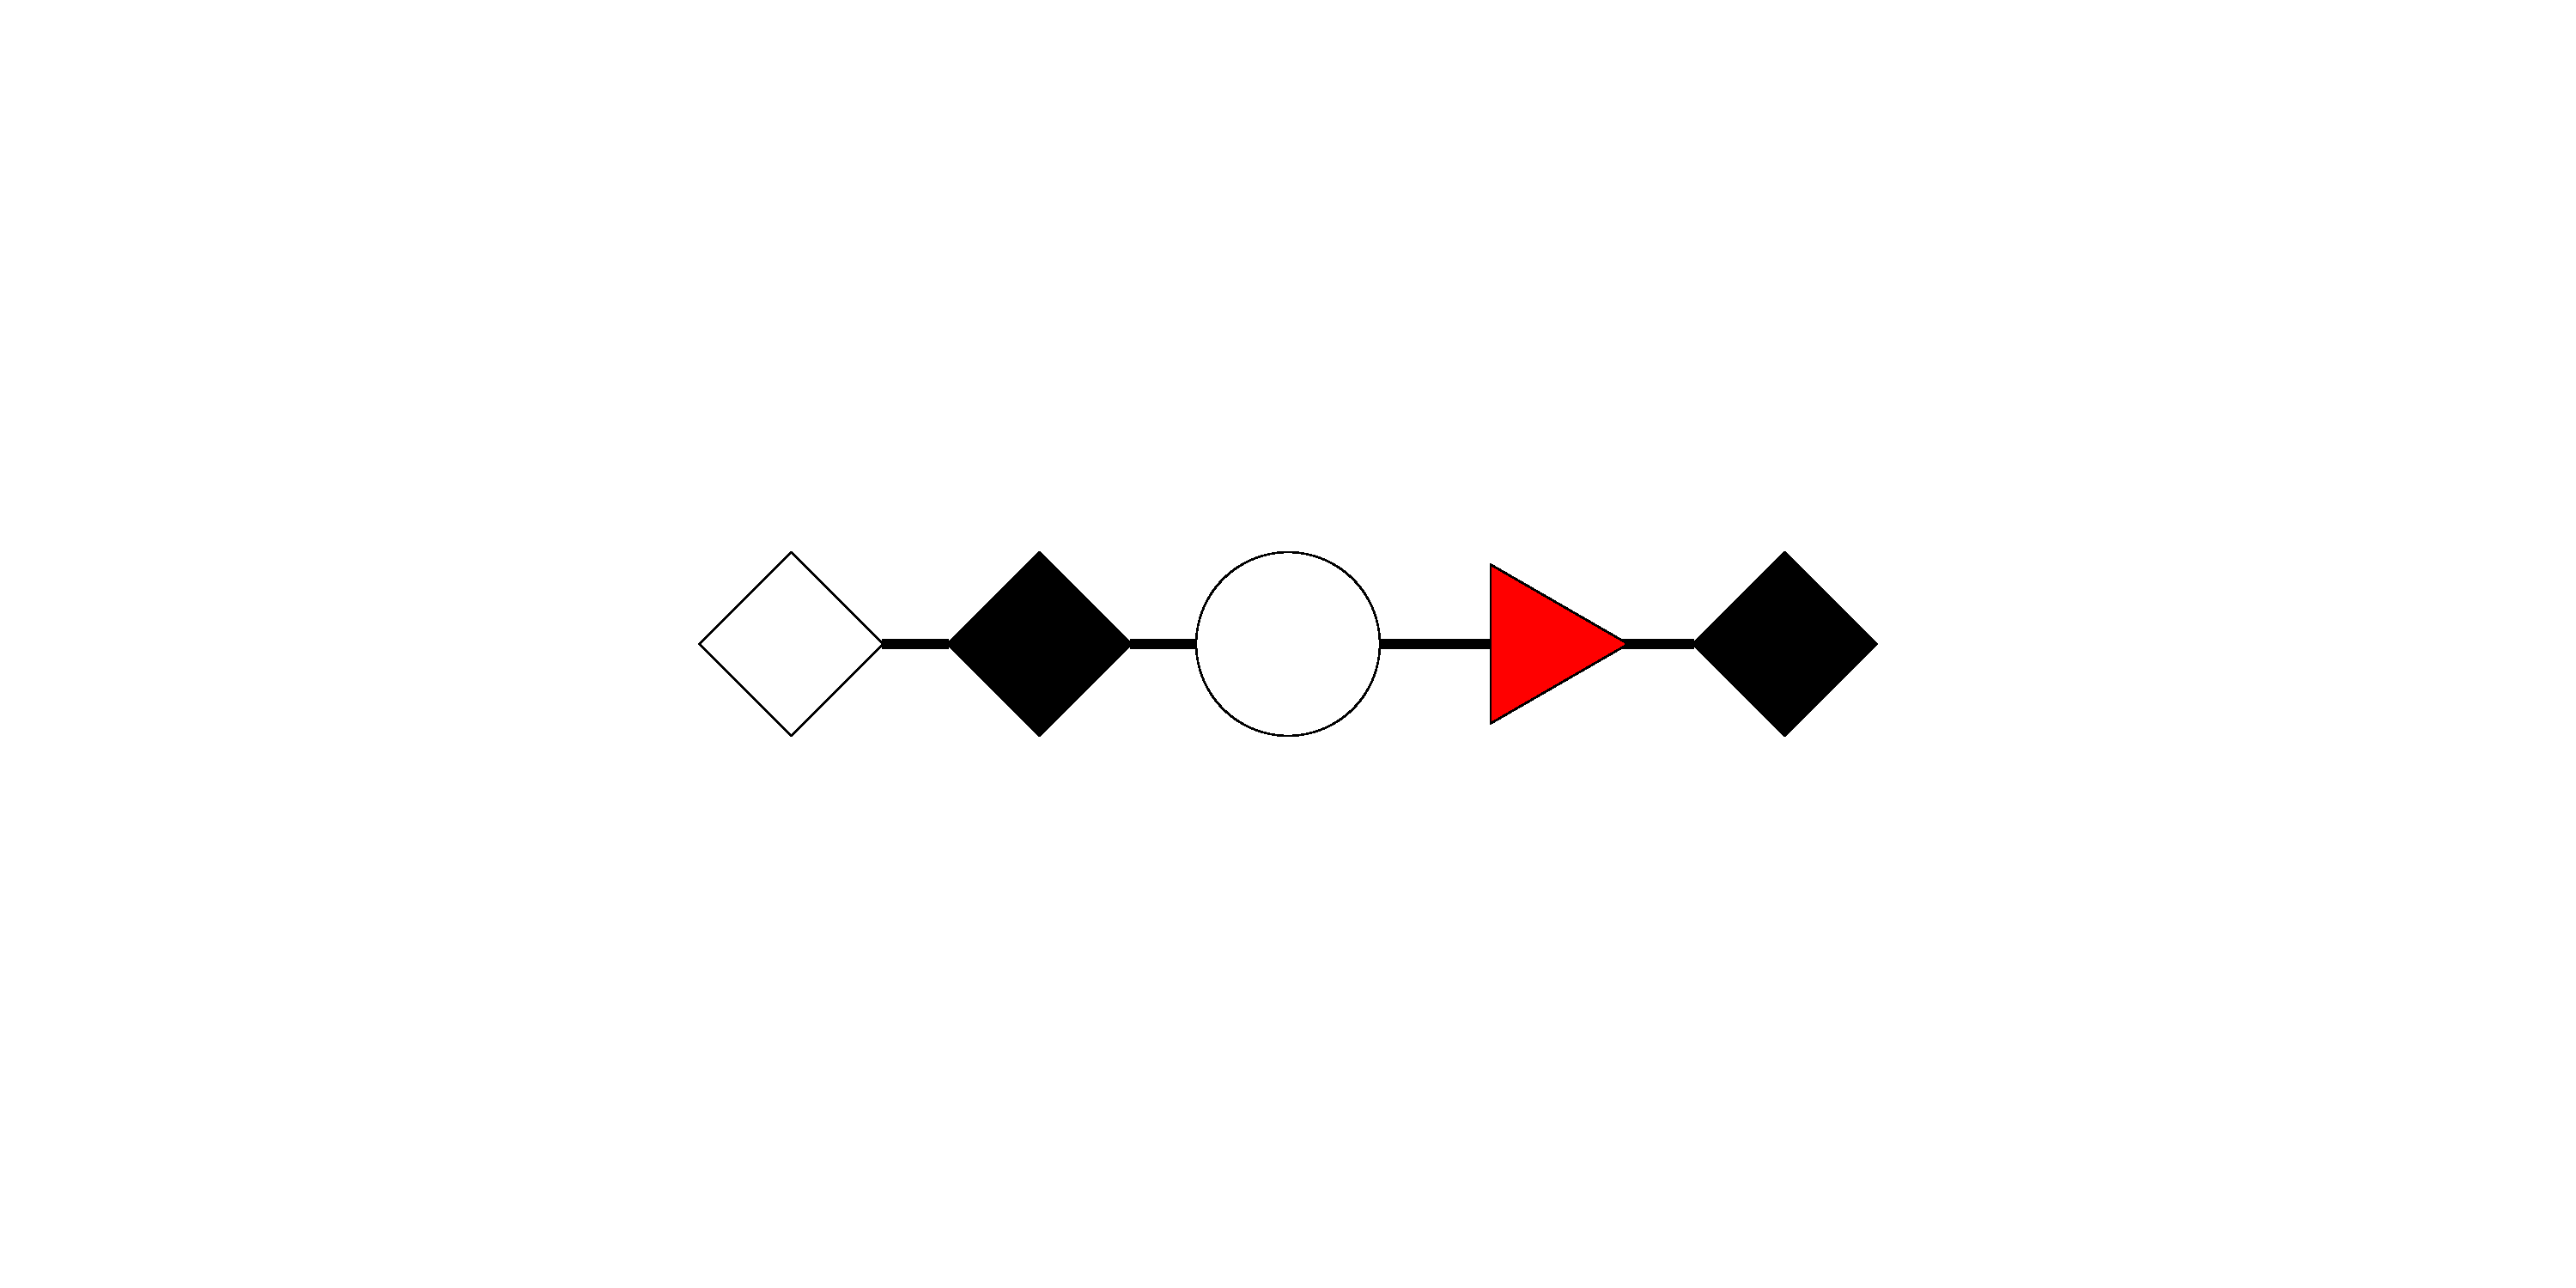
\includegraphics[scale=.225,clip=true,trim = 13cm 10cm 13cm 10cm]{./images/effect_constant_twohops} &  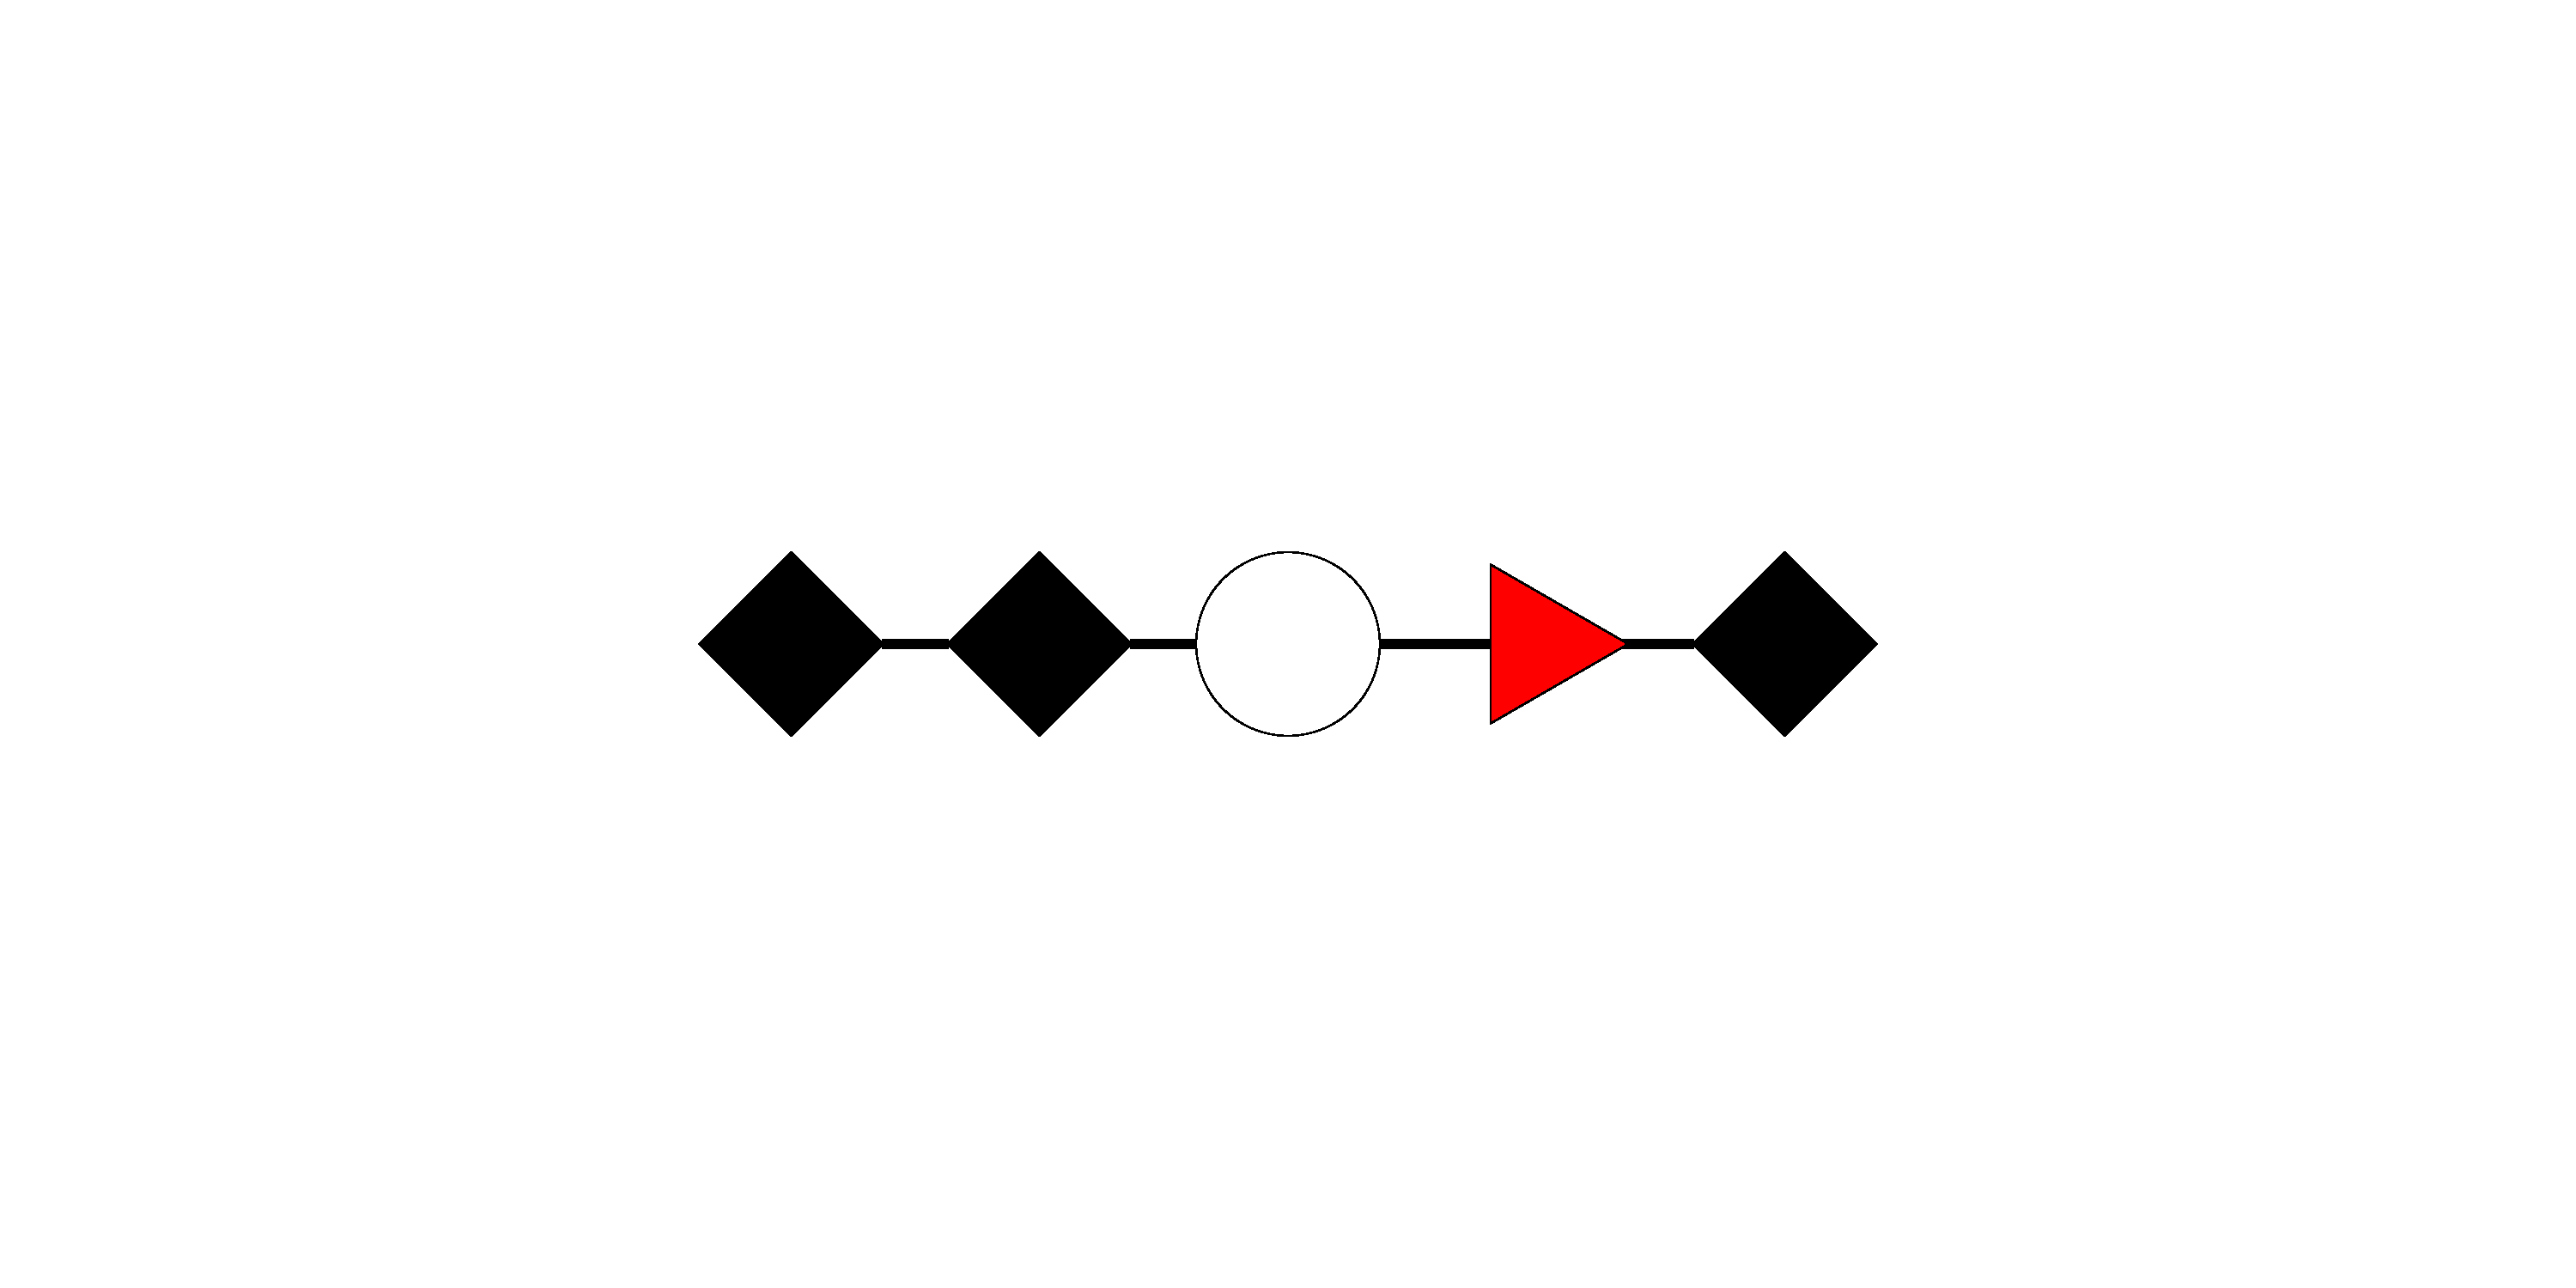
\includegraphics[scale=.225,clip=true,trim = 13cm 10cm 13cm 10cm]{./images/effect_constant_threehops} \\ \hline 
Decaying effect &  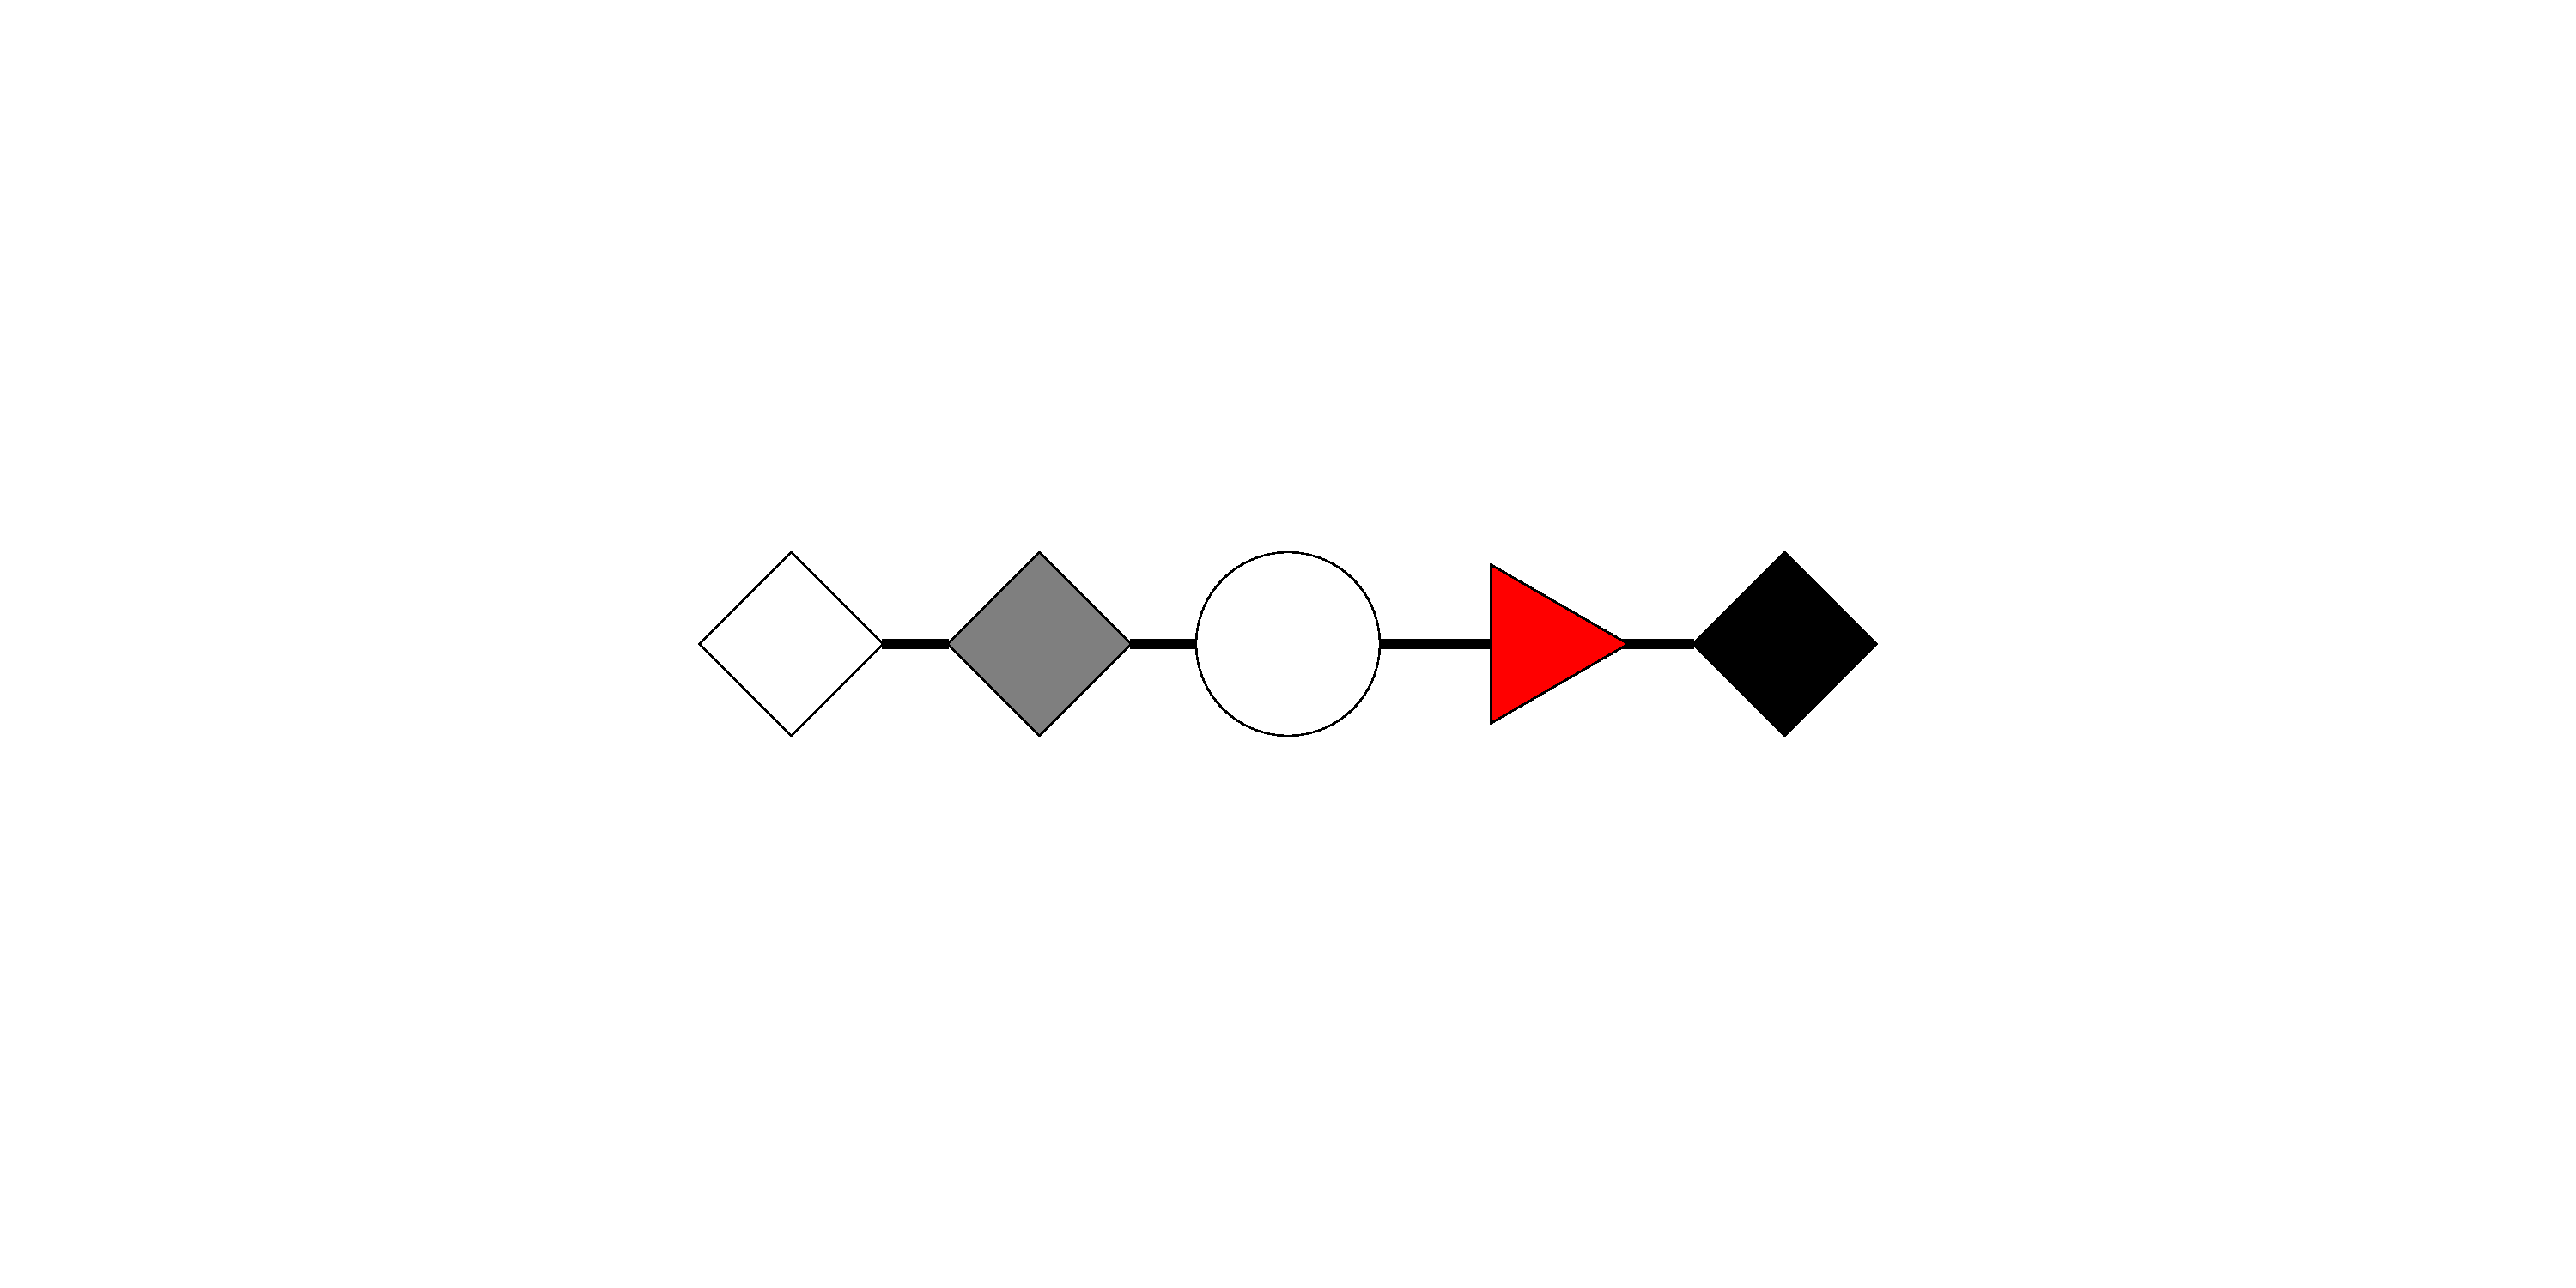
\includegraphics[scale=.225,clip=true,trim = 13cm 10cm 13cm 10cm]{./images/effect_decay_twohops} &  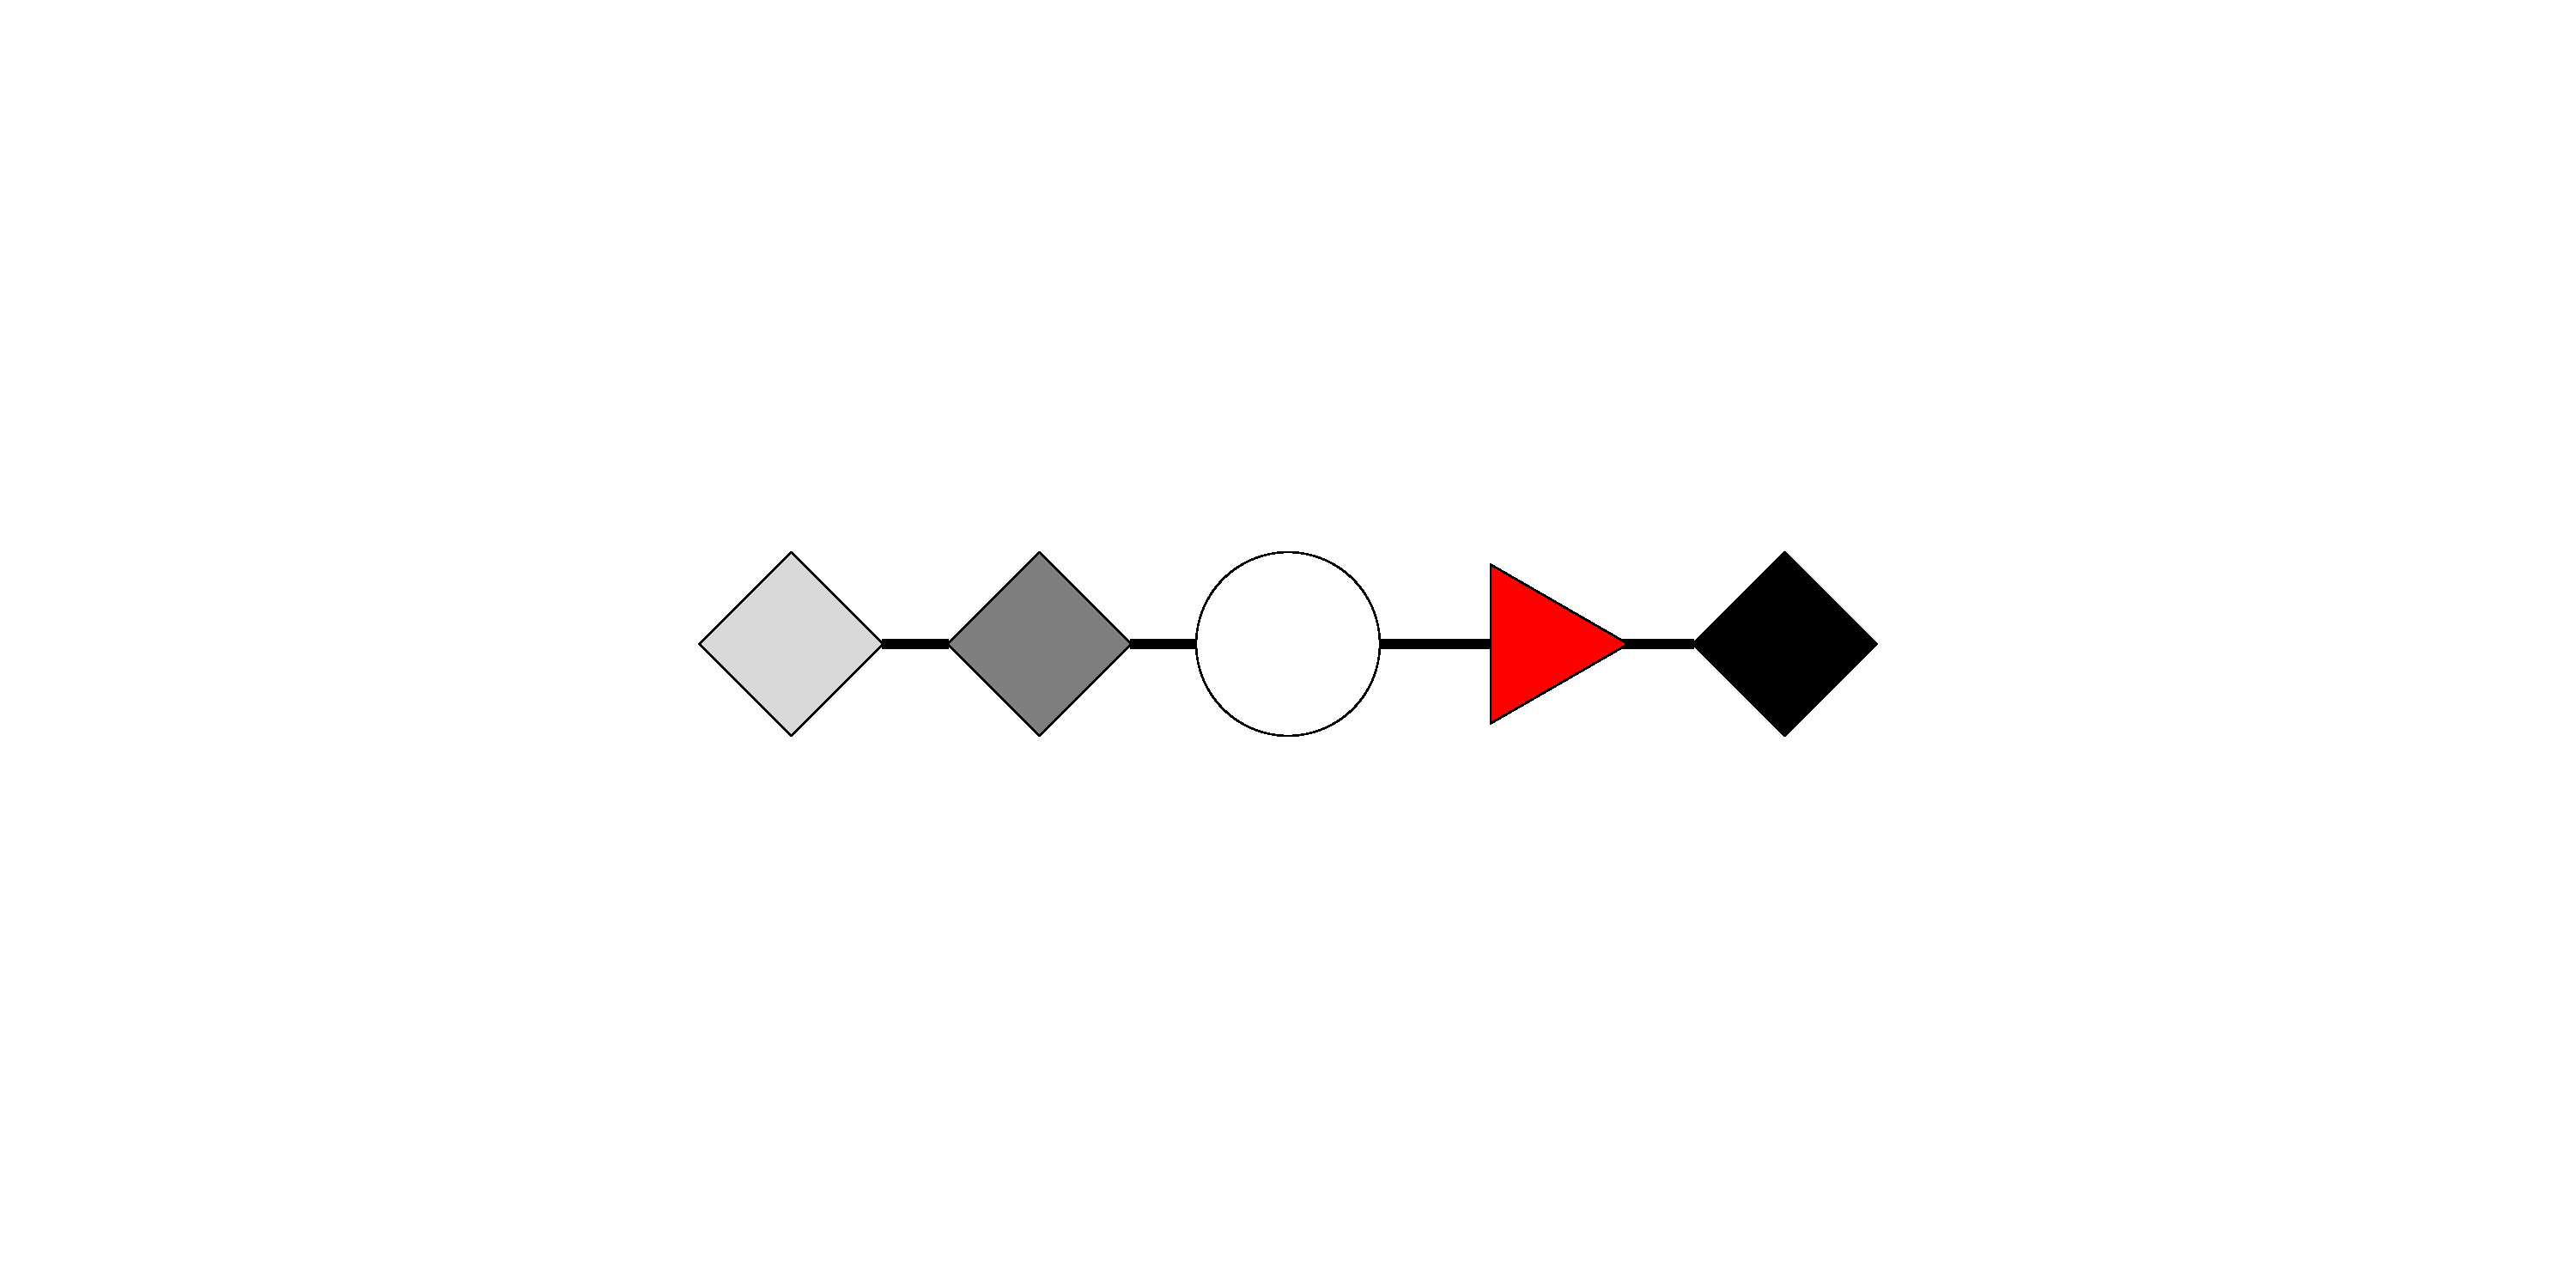
\includegraphics[scale=.225,clip=true,trim = 13cm 10cm 13cm 10cm]{./images/effect_decay_threehops} \\
\hline 
\end{tabular}

\caption{Alternative models of effects, focusing on a single focal node. The red triangle represents the focal node, on which the other nodes have various effects under each model. Square nodes are treated. The circle is a control node. The darker the node's shading, the larger the effect it has on the focal node.}
\label{tab:fourmodels}
\end{table}

\subsubsection{Neighborhood selection}

Once the researcher decides which network---or combination of networks---to use in analysis, it is important to determine the neighborhood within which the effects of the treatment can be transmitted. For example, \cite{Bond:2012} find that Facebook users' voter turnout, as expressed on their Facebook walls, influences not only their Facebook friends' turnout decisions, but also turnout of the friends of their friends. This means that the effects of a Facebook user's turnout decision spread within a neighborhood of two hops through the friendship network. This specification decision becomes more complicated when the network is weighted (i.e., ties can take on many values rather than just being binary tie/no tie), as in the legislative networks that we consider in our applications. In the weighted network case transmission is likely a function of connection strength, but may also disappear at some threshold (e.g., the level of ideological distance that indicates opposition between two legislators).  In our consideration of state legislative networks, we specify the neighborhood in two ways when using the ideological similarity networks:
\begin{itemize}
\item Entire network: Treatment effect can propagate through the entire network---proportional to ideological similarity---to affect the outcome of control units. 
\item K-nearest neighbors: Treatment effects can spread to control units from their K nearest neighbors, varying the value of K.
\end{itemize}

The definition of neighborhood depends on substantive knowledge about the interaction in a certain network. For example, a state legislature is a relatively small and internally familiar community. As such, everyone may potentially communicate with everyone else regarding major legislative tasks and actions. However in looking at interpersonal political communication networks among regular citizens, even the closest of friends may fail to communicate about an election or other major political event.


 \subsubsection{Interference effect specification}:
The above two specifications---selecting the network and the neighborhood---determine which units play a role in the interference reflected in the hypothesized model. Diffusion model specification involves defining how the treatment effect spreads through the network. We highlight two considerations---the way in which treated and untreated neighbors factor into the interference effects, and the linearity of the interference model. 

The first consideration regards whether a control unit influenced by the number of treated units with which it interacts (e.g., as in an epidemic network), or by the balance or proportion of its neighbors that are treated (e.g., as we would assume in a voting or opinion-spreading network). \citet{bowers2012reasoning} specification assumes treatment spreads as a function of the number of treated neighbors. Alternatively, the Voter Model---a classic mode of opinion dynamics in networks---assumes that the proportion of treated neighbors is the relevant quantity \citep{valentini2014self}. This specification choice likely comes down to whether the researcher assumes that the treatment and the lack of it are equally powerful forces, or whether change in the outcome can only result from exposure to treated units. If untreated neighbors can offset the effects of treated neighbors, it is likely the proportion that matters. If units are influenced only by treated neighbors, it is likely the raw count of treated neighbors that is relevant. 

Though a very familiar consideration in quantitative social science, functional form assumptions are also relevant in the specification of a model of network effects. It is important to determine whether the functional form of the propagation of treatment effect should be linear or non-linear. Does the second treated neighbor have the same effect on a node's outcome as the first treated neighbor, or does the effect diminish? Or, alternatively, is it a threshold effect that only manifests when the number of treated neighbors reaches a critical level (e.g., a model in which a unit adopts the majority opinion among its neighbors)? \citet{coppock2014information} adopts a linear functional form in specifying the way in which legislators learning about their districts' opinions effects the votes of ideologically similar legislators. Alternatively, the classic susceptible-infected-recovered (SIR) model in epidemiology assumes a model in which the probability of transmission increases at a decreasing rate with the number of exposed neighbors to which a unit is exposed \citep{dodds2004universal}.


%\item \textbf{Test statistics selection}: To evaluate differences across experimental conditions using the framework of \citet{bowers2012reasoning}, the researcher must select a test statistic to evaluate the differences in terms of the hypothesized model of effects. As discussed earlier, \citet{bowers2012reasoning} uses the KS test statistics, which is problematic for categorical responses, especially those with three or more experimental categories. The test statistic used by  \citet{coppock2014information}---the sum of squared errors from a linear probability model of the binary outcome---is an option for managing categorical outcomes. The Anderson-Darling test is an alternative to the KS test with multiple experimental categories \citep{anderson1954test}. Other possible tests include the Mann-Whitney U and Control Median tests \citep{rosenbaum2012interference}.






%%%%
\section{Replication Analyses: Testing for Network Effects}
%%%%

To illustrate testing for effects via network models of effects, we re-analyze results from two field experiments on state legislatures. Our application builds directly on \citet{coppock2014information}. Since it is generally infeasible to recruit legislators for lab experiments, field experiments represent the best option for design-based causal identification of effects in research on legislative behavior. The literature offers many recent examples of field experiments in legislative studies \citep[e.g., ][]{bergan2009does,butler2011politicians,butler2012field,broockman2013black,nyhan2015effect,bergan2015call}. In these experiments, the researcher introduces a manipulation (e.g., a communication from a constituent, or information about constituent preferences), and then observes legislators' behavior in terms of casting roll call votes or reacting to the communication on an individual basis. Since legislators regularly communicate and collaborate, it is highly possible that SUTVA is violated in a legislative field experiment. Note, our replications are not intended to serve as a meta analysis of interference in legislative field experiments, or to provide evidence regarding whether there is or is not interference in state legislatures, generally speaking. Rather, the purpose of the replications is to illustrate the considerations, steps, and process of testing for interference using the data produced by the experiments we replicate. 

In each of the replications and extensions that follow, we test causal models that include network effects. In order to test these models, we must specify their functional forms and select the data to use in measuring the network. For each replication, we consider multiple definitions of both the network and the neighborhood through which network effects are transmitted, as we do not have strong prior expectations regarding exactly which network or neighborhood should be included in the models of effects. 

We make specification choices in terms of both linearity of the model of effects and the effects of control units that are based in theoretical considerations. First, in terms of the linear functional form of the model of effects, we stick with a linear model due to (1) the relatively small datasets with which we are working, and (2) the dichotomous nature of the outcome variables in each experiment. Since the datasets are small there is a significant degrees-of-freedom cost in adding additional parameters to the model of effects, and making the model nonlinear would require adding a parameter that controlled the shape of the curve. The fact that the outcome variable is dichotomous in each experiment also limits the information---in terms of variability---that could be used to identify the functional form of the model of effects. In terms of of the effects of controls (i.e., number vs proportion of treated neighbors), we assume that the number of treated neighbors is the relevant quantity in each application.  In each of the experiments we replicate, treated legislators are provided with a form of communication that could, in theory, be passed along to other legislators. Further, the likelihood that this information will be passed along should increase with the number of treated legislators in a legislator's neighborhood. Lastly, in the replications we consider the treatments include informational communications and requests for action, but control units are not provided with either information or requests that counteract that provided to treated units. As such, we do not expect to see any balancing effect between treated and control units.

We present each replication in a separate section below. For each analysis, we visualize the plots of p-values from the test of the model of effects at the specified parameter values. Using the framework of \citet{bowers2012reasoning}, the point estimate is the estimate that results in the maximal p-value. We provide tables of point estimates and confidence intervals. The 95\% confidence interval is given by the region that includes p-values greater than 0.05.

\subsection{\citet{butler2011can}}

\begin{itemize}
\item Ideological distance network and top 30\% 
\item Same party and committee network---direct ties and 1/geodesic distance
\item cohort network--same cohort, two hops cohort 1/2 effect
\end{itemize}

Butler and Nickerson conducted an experiment on New Mexico legislators to study the effect on legislators of learning public opinion from their constituencies. In 2008, a special session of the New Mexico State Legislature was called to vote on a bill regarding proposed spending plans for a budget surplus---a tax rebate. Butler and Nickerson conducted a large-scale phone survey to gather constituent opinions from across the state. Using matched-pair randomization---matching in terms of political party, 35 out of 70 legislators were assigned to the treatment group. Legislators in the treatment group were sent a letter containing the district-specific support for the proposed spending plan in their own districts. The original paper conducts a direct comparison of outcomes across treatment and control group.  They find that the effects of the treatment on legislators' votes were conditioned by the level of support for the measure indicated in the treatment message. In districts with high support for the tax rebate, the treatment had little effect. This is because legislators generally assumed that the tax rebate would be popular, and that constituents would support the measure. In districts with low support for the tax rebate, the treatment had a negative effect on the likelihood of voting in support for the measure. 

\citet{coppock2014information} applied the \citet{bowers2012reasoning} methodology to test for propagation of treatment in this experiment. The indirect effect estimates were not statistically significant \citep{coppock2016information}, even when separating the sample into low and high support districts. As detailed in Section 3, Coppock used a network based on ideological similarity, where the legislator's outcome is affected by every other legislator in the network, but with varying weight based on ideological similarity. Coppock used a linear model to represent the direct and indirect effects of the treatment on the outcome. We begin by replicating this analysis. {\bf SAYALI, NEW DESIGN TO DESCRIBE HERE} In the extension, we consider two types of networks--- one based on ideological similarity and the other on serving on committees together. We also vary the neighborhood specification to consider an effect from all other legislators---proportional to ideological distance or effect only from k-nearest neighbors. Results of this analysis are presented in section 6.1. The following list summarizes the steps taken to implement Coppock's analysis of interference in the \citet{butler2011can} replication. Note that we re-use these steps in the other replication analyses where the similarity scores are replaced with the respective definition of the network and neighborhood.

\begin{enumerate}
\item Calculate W-NOMINATE ideology score for each legislator using roll call vote data

\item Calculate ideological similarity as $Similarity_{i,j} = \frac{2 - |ideo_i - ideo_j|}{2}$

\item Calculate raw exposure as $Raw\; exposure_i =  \sum_{j=1}^{n}Similarity_{i,j} * z_j, \; j \neq i$. 

\item Coppock introduces an adjustment for the expected exposures of legislators. Exposures are simulated under a large number of randomizations. Each randomization where legislator \textit{i} is in treatment is indexed as \textit{k} (\textit{k} = 1, 2, ..., K) and where legislator \textit{i} is in control is indexed as \textit{l} (\textit{l} = 1, 2, ..., L) $$Expected \; exposure_{i, z_i=1} =  \frac{\sum_{k=1}^{K}\sum_{j=1}^{n}Similarity_{i,j} * z_{j,k}}{K}, \; j \neq i, \; z_{i,k}=0$$ $$Expected \; exposure_{i, z_i=0} =  \frac{\sum_{l=1}^{L}\sum_{j=1}^{n}Similarity_{i,j} * z_{j,l}}{L}, \; j \neq i, \; z_{i,l}=1$$

\item Using the hypothesized parameter values, remove  the model of effects based on a linear regression.

\item Regress hypothesized uniformity trials on direct and indirect treatment, and use the residual sum of squares (RSS) as test statistic. See\citet{bowers2016research} for discussion of why this is an appropriate test statistic for this framework.

\item The p-value for each hypothesized treatment effect is the proportion of simulated RSS that is lower than the observed RSS (note that smaller RSS indicates more variance explained).
\end{enumerate}

One last detail of implementing the Bowers et al. hypothesis testing framework regards the grid of hypothesized parameters over which p-values are calculated. Since the testing process does not involve an optimization routine, there is no way for the parameter values to be selected automatically. However, standard optimization methods can be used to approximate point estimates around which to expand the grid of hypothesized values. In our applications, the model of effects has a linear form, and we can use linear regression to find the estimates around which to expand the grid. In terms of how far to expand the grid----there should be enough grid points that none of the confidence interval boundaries lies at a boundary of the grid of hypothesized parameters.

\subsubsection{Results for \citet{butler2011can} data}

The results of our analyses are presented in the form of heat maps displaying the full range of parameter values considered, and tables in which we present the point estimates and 95\% confidence intervals for the estimates. The dependent variable in this application is coded as nay=0, yea=1.The p-value plot for replication of the main analysis in \citet{coppock2014information} is in Figure 1. The p-value is highest (~0.997) when the direct effect is -0.25 and indirect effect is -0.15. Negative effects indicate that the treatment reduced the likelihood of voting in favor for those who received the treatment directly as well as those to whom it propagated, due to ideological similarity. The negative effects discovered in this experiment may be attributable to the assumed popularity of the bill. A treatment survey that indicated a high level support had no effect on legislators who were already planning to vote for the bill. However, low or moderate support on a treatment survey may have changed the minds of those legislators who were planning to support the bill. Confidence intervals are drawn using dashed lines. Neither the indirect nor the direct effects are statistically significant at the 0.05 level since each confidence interval contains zero. This is not a surprising result, as the direct effects reported in the original paper were not statistically significant at the 0.05 level.

\begin{figure}
	\centering
	\begin{tabular}{cc}
	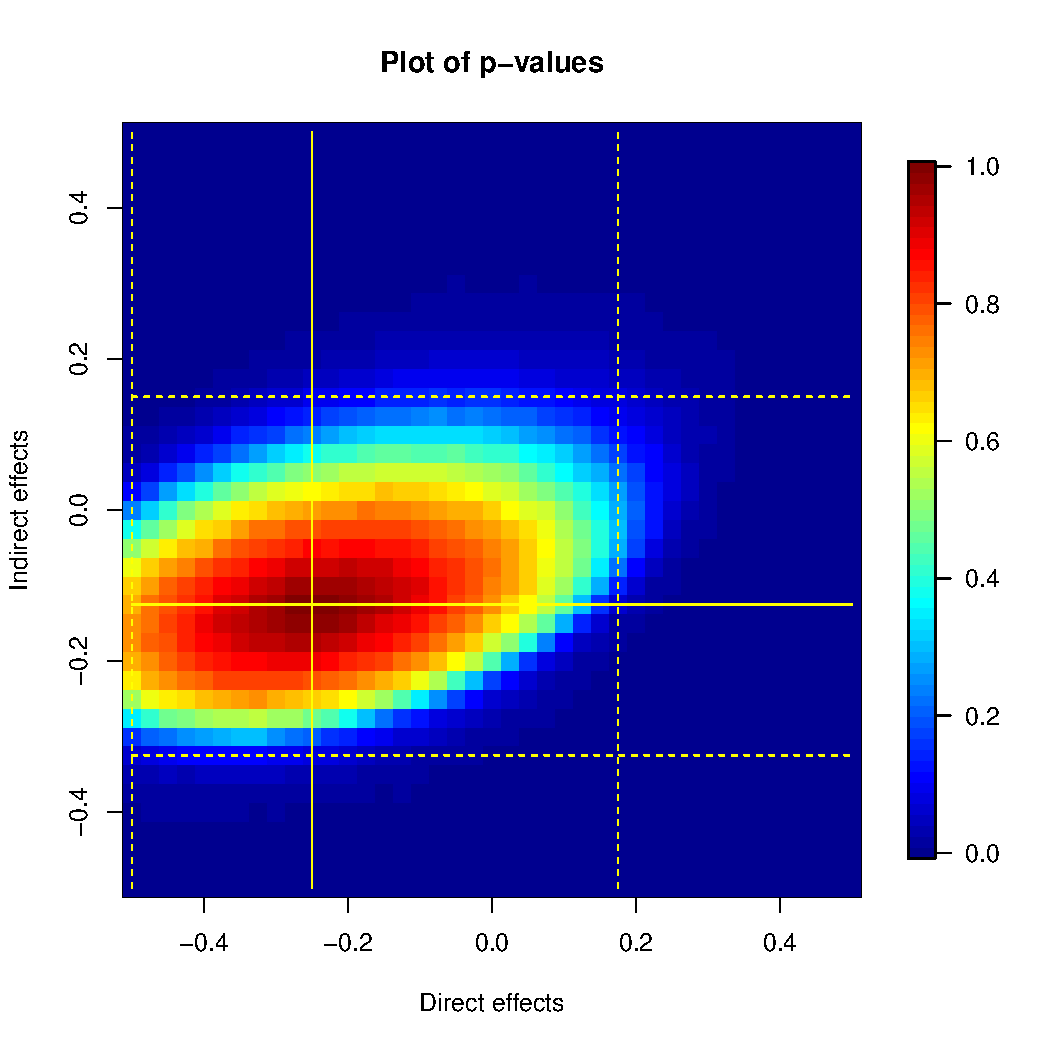
\includegraphics[scale=0.45]{./images/pval_plot_coppock_replication.pdf}
	\end{tabular}
	\caption{Main analysis for \citet{butler2011can} data}
\end{figure}


The first extension we consider is a change in the neighborhood specification. Instead of looking at ideological similarity across the network,  we consider only the nearest k neighbors at values k = 3,5,8,12.  For this network, ideological similarity is replaced with a 1 if $j$ is one of $i$'s $k$ nearest neighbors, and 0 otherwise. In Figure 2, we see that the direct and indirect effects which maximize the p-value, are lower in magnitude than those in the first specification. When we model interference between all legislators in the network, we observe higher spillover than when looking at only nearest neighbors. We see that the observed indirect effect is higher when considering a a broader neighborhood (the entire network being the broadest neighborhood we can consider).  Interestingly, we only see a result that is statistically significant, based on the 95\% confidence interval, when looking at the indirect effect with a neighborhood defined as the twelve nearest neighbors. Overall, our finding of negative spillover through the ideological network is robust to neighborhood specification, but the estimates are not generally statistically significant.
 

\begin{figure}
	\centering
	\begin{tabular}{cc}
	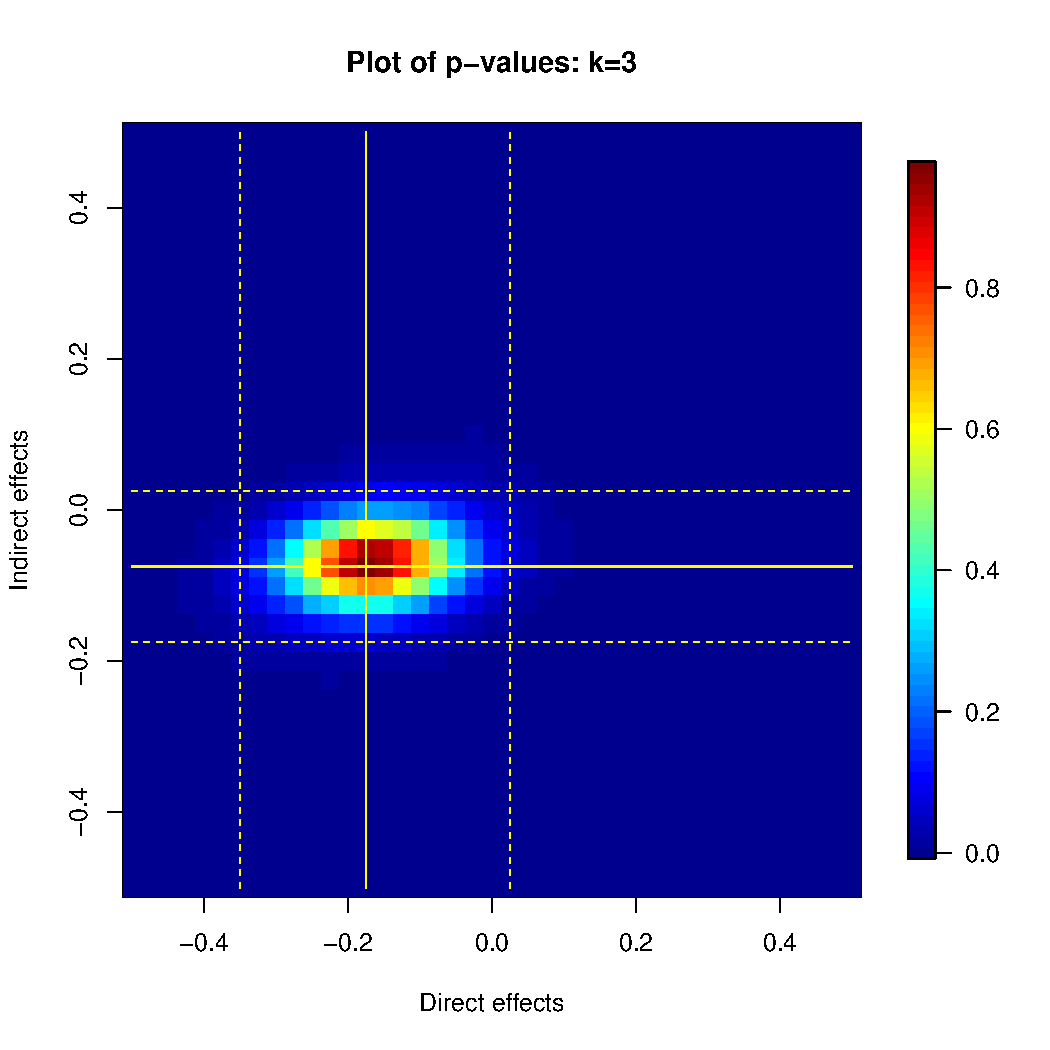
\includegraphics[scale=0.45]{./images/pval_plot_coppock_ideo_3nn.pdf} &
	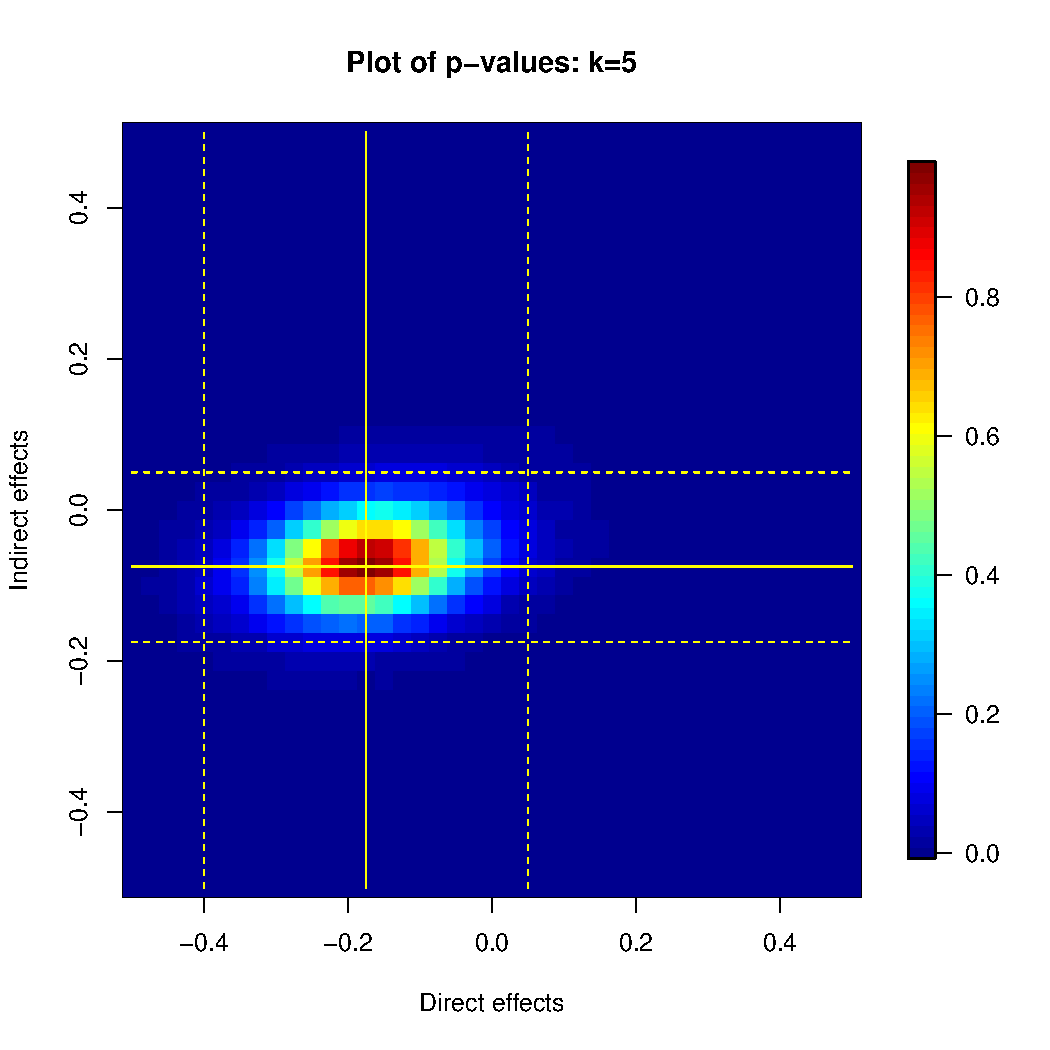
\includegraphics[scale=0.45]{./images/pval_plot_coppock_ideo_5nn.pdf} \\ 
	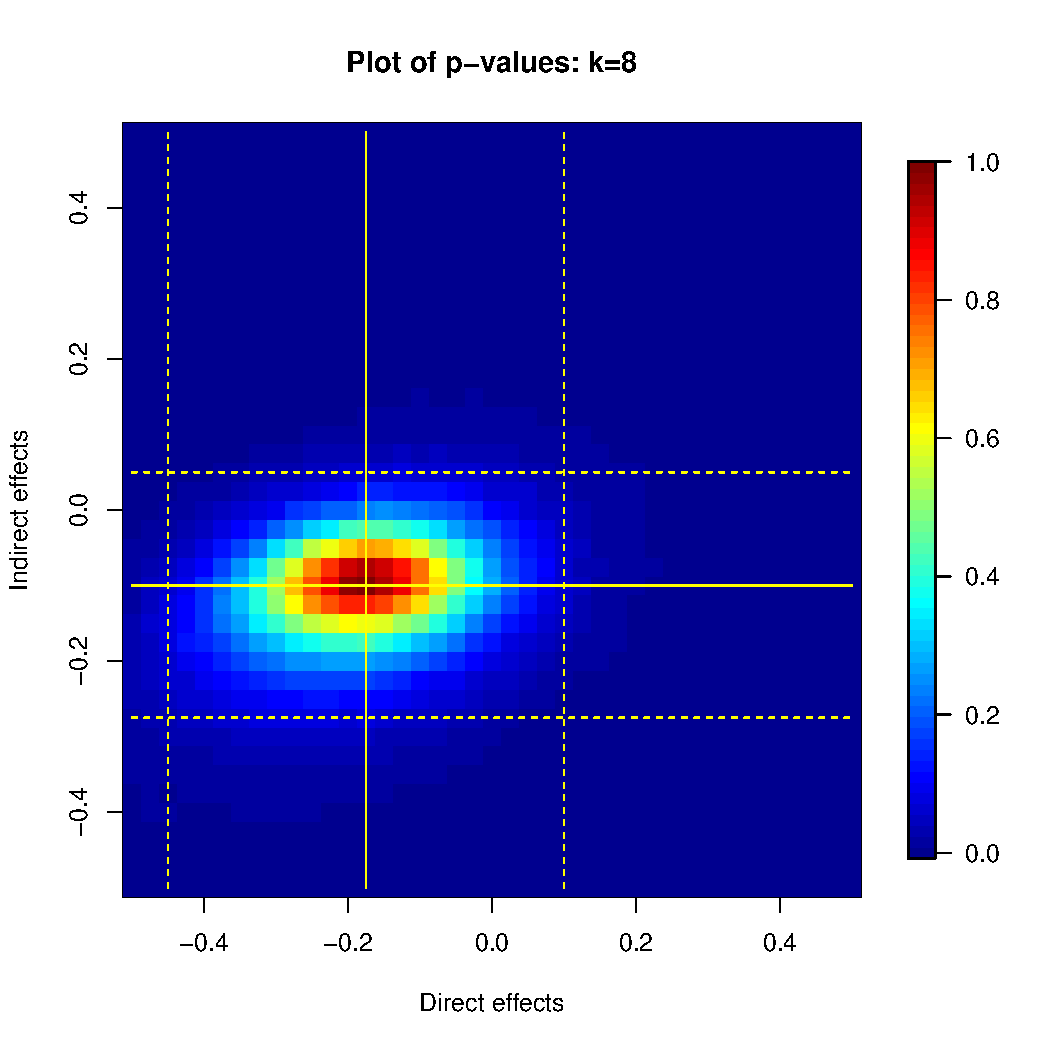
\includegraphics[scale=0.45]{./images/pval_plot_coppock_ideo_8nn.pdf} &
	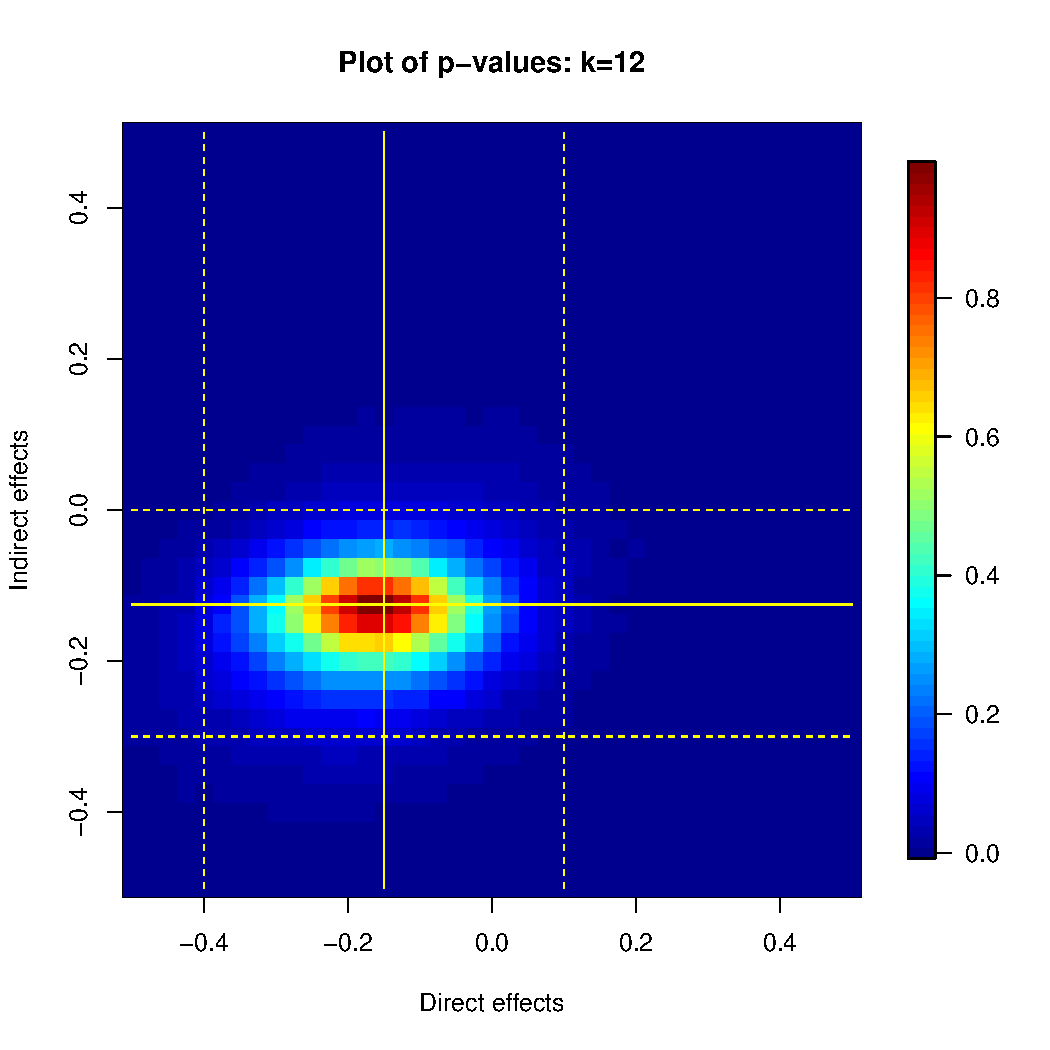
\includegraphics[scale=0.45]{./images/pval_plot_coppock_ideo_12nn.pdf} \\ 
	\end{tabular}
	\caption{k-nearest ideological neighbors for \citet{butler2011can} data}
\end{figure}


In the next extension we change the network to look at co-committee membership as defining the ties through which interference occurs.\footnote{Records of standing committee membership in the 16 standing committees in place during the 2008 regular session was obtained by email correspondence with the New Mexico Legislative Council Service Librarian.}  An undirected edge exists between legislators who served on standing committees together.  We define the network at two thresholds---serving on at least one committee together and serving on at least two committees together. Results indicate that the committee network does not carry the effect of treatment to control units, as the point estimate is zero. The point estimate for the direct effect is still negative with the committee network.

\begin{figure}
	\centering
	\begin{tabular}{cc}
	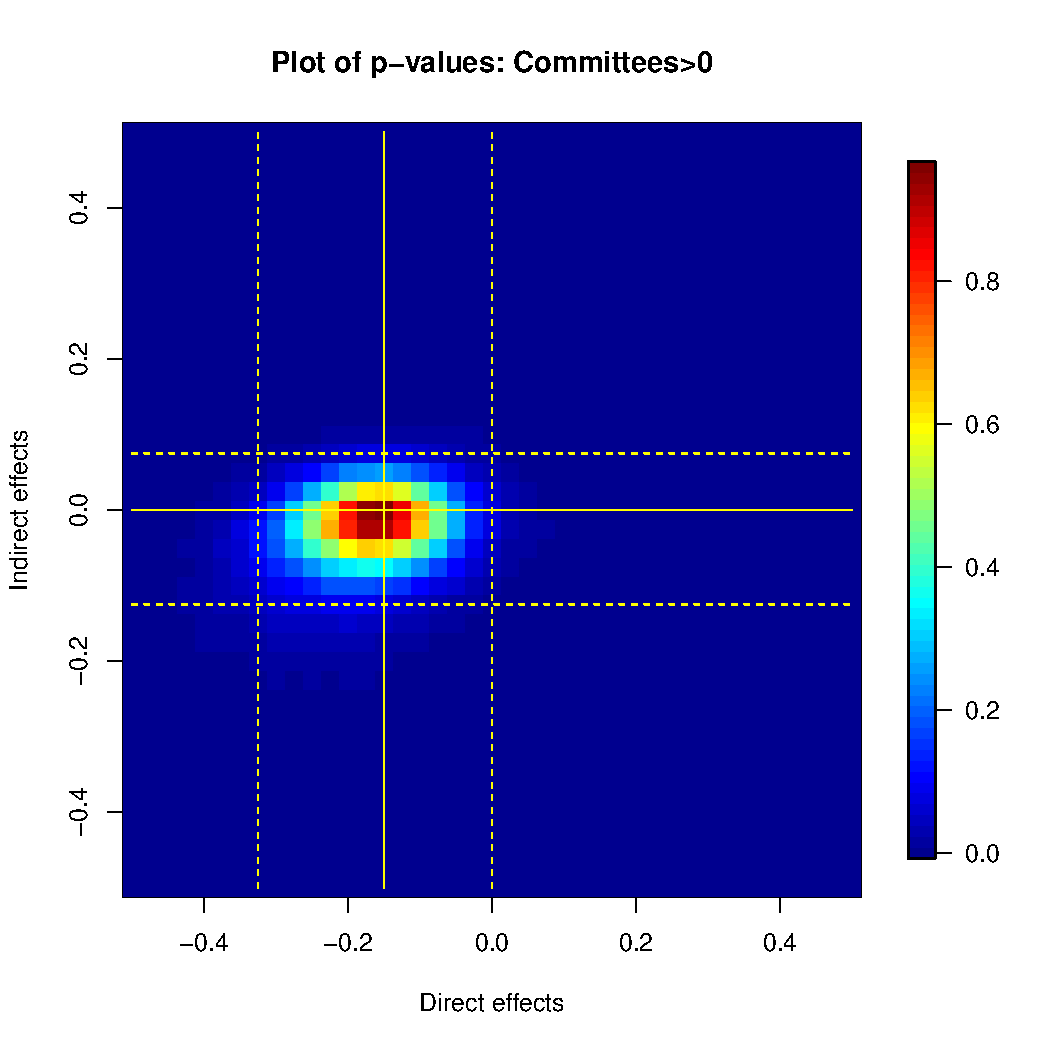
\includegraphics[scale=0.45]{./images/pval_plot_coppock_committee_1ormore.pdf} &
	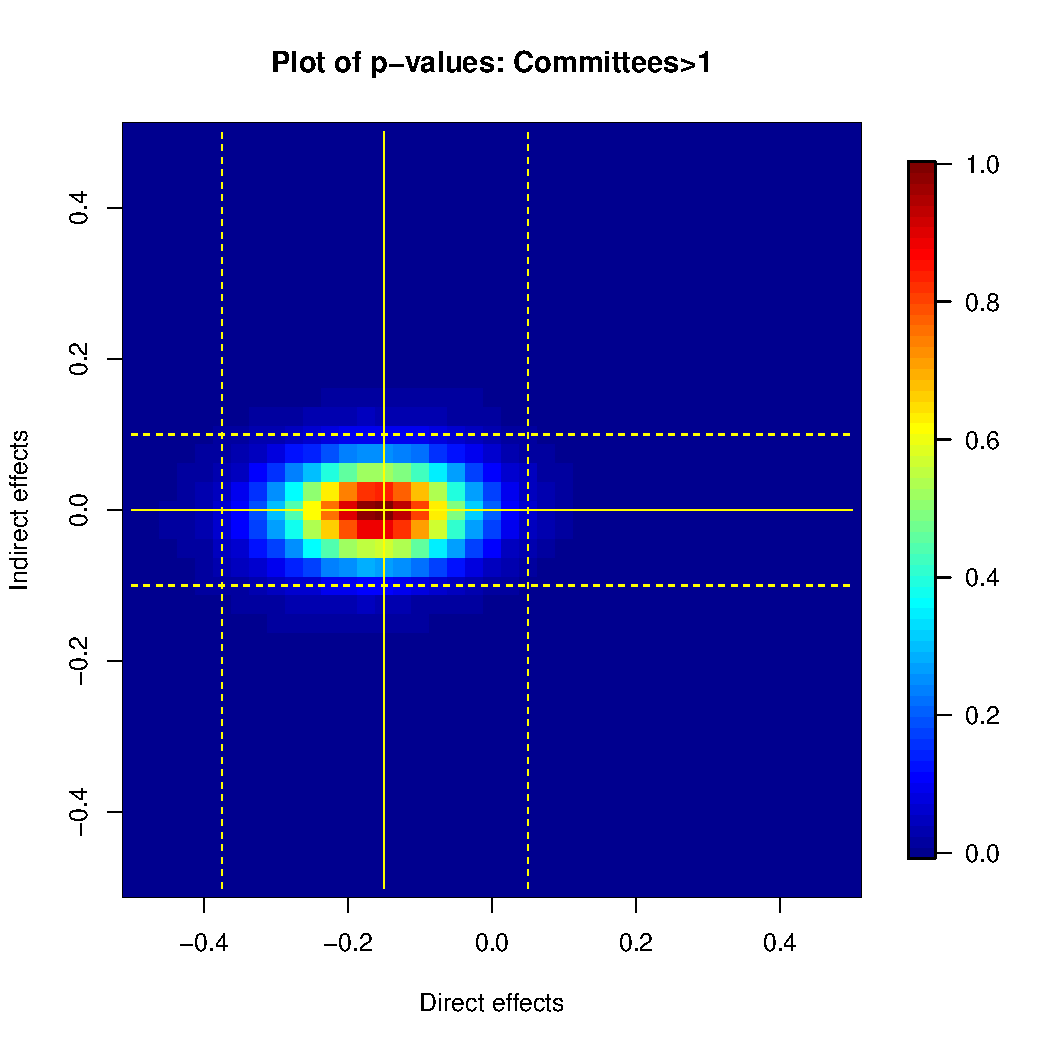
\includegraphics[scale=0.45]{./images/pval_plot_coppock_committee_2ormore.pdf}
	\end{tabular}
	\caption{Committee network for  \citet{butler2011can} data}
\end{figure}


\floatsetup[table]{objectset=centering,capposition=top}
\begin{table}[h]
\centering
\begin{tabular}{lcccc}
\toprule
\multirow{2}{*}{Model} & \multicolumn{2}{c}{Direct effect} & \multicolumn{2}{c}{Indirect effect} \\
\cmidrule(l){2-3} \cmidrule(l){4-5}
 & Estimate & 95\% CI & Estimate & 95\% CI \\
\midrule
Ideology: full network  & -0.25 & (-0.5, 0.175) & -0.15 & (-0.325, 0.15)\\
Ideology: 3nn & -0.175 & (-0.35, 0.025) & -0.075 & (-0.175, 0.025)\\
Ideology: 5nn & -0.175 & (-0.4, 0.05) & -0.075 & (-0.175, 0.05)\\
Ideology: 8nn & -0.175 & (-0.45, 0.10) & -0.10 & (-0.275, 0.05)\\
Ideology: 12nn & -0.15 &(-0.4,  0.1) & -0.125 & (-0.3, 0)\\
Committee: >0& -0.15 & (-0.325, 0) & 0 & (-0.125, 0.075)\\
Committee: >1 & -0.15 & (-0.375, 0.05) & 0 & (-0.1, 0.1)\\
\bottomrule
\end{tabular}
\caption{Results from \citet{coppock2014information} data}
\end{table}


% Same table as above with raw/unadjusted/unstandardized effects
%\floatsetup[table]{objectset=centering,capposition=top}
%\begin{table}[h]
%\centering
%\begin{tabular}{lcccc}
%\toprule
%\multirow{2}{*}{Model} & \multicolumn{2}{c}{Direct effect} & \multicolumn{2}{c}{Indirect effect} \\
%\cmidrule(l){2-3} \cmidrule(l){4-5}
% & Estimate & 95\% CI & Estimate & 95\% CI \\
%\midrule
%Ideology: full network  & -0.175 & (-0.35, -0.025) & -0.075 & (-0.5, 0.5)\\
%Ideology: 3nn & -0.175 & (-0.35, 0.025) & -0.05 & (-0.175, 0.025)\\
%Ideology: 5nn & -0.175 & (-0.4, 0.025) & -0.075 & (-0.2, 0.025)\\
%Ideology: 8nn & -0.175 & (-0.45, 0.1) & -0.075 & (-0.325, 0.05)\\
%Ideology: 12nn & -0.2 &(-0.45,  0.05) & -0.15 & (-0.375, -0.025)\\
%Committee: >0& -0.15 & (-0.3, 0) & -0.025 & (-0.275, 0.3)\\
%Committee: >1 & -0.15 & (-0.03, 0) & -0.025 & (-0.2, 0.15)\\
%\bottomrule
%\end{tabular}
%\caption{Results from \citet{coppock2014information} data: Raw exposure for all analysis except Full Ideological Network}
%\end{table}


\subsection{\citet{bergan2015call}}


The second dataset we work with comes from an experiment on the Michigan state legislators. This experiment was conducted on legislators from both houses, in the context of anti-bullying legislation. Legislators were stratified based on various background variables. The treatments were calls from constituents expressing their support for the proposed bill. Treatment was given in three different doses, which differed in the number of calls places to the given legislator. Once again, the authors conducted an analysis under SUTVA and concluded that this treatment has a significant effect on the final vote on the bill. They observed a 12 percentage point increase in the likelihood of voting in favor of the anti-bullying bill, for those treated. Table 2 summarizes results of the \citet{bergan2015call}. 

This data has not been analyzed for indirect effects previously. However, for all the reasons that we would expect to see interference in the \citet{butler2011can} results, we would expect to see them in the \citet{bergan2015call} results. We conduct an analysis that is analogous to that in \citet{coppock2014information}, where a network is constructed based on ideological scores of legislators, using roll call data. We do not find evidence of indirect effects via this network. It is possible that we can attribute this to the nature of the bill.  Voting behavior on an anti-bullying bill may not be governed by ideological coalitions. Figure 4 shows the plot of p-values for this analysis.

\begin{figure}
	\centering
	\begin{tabular}{cc}
	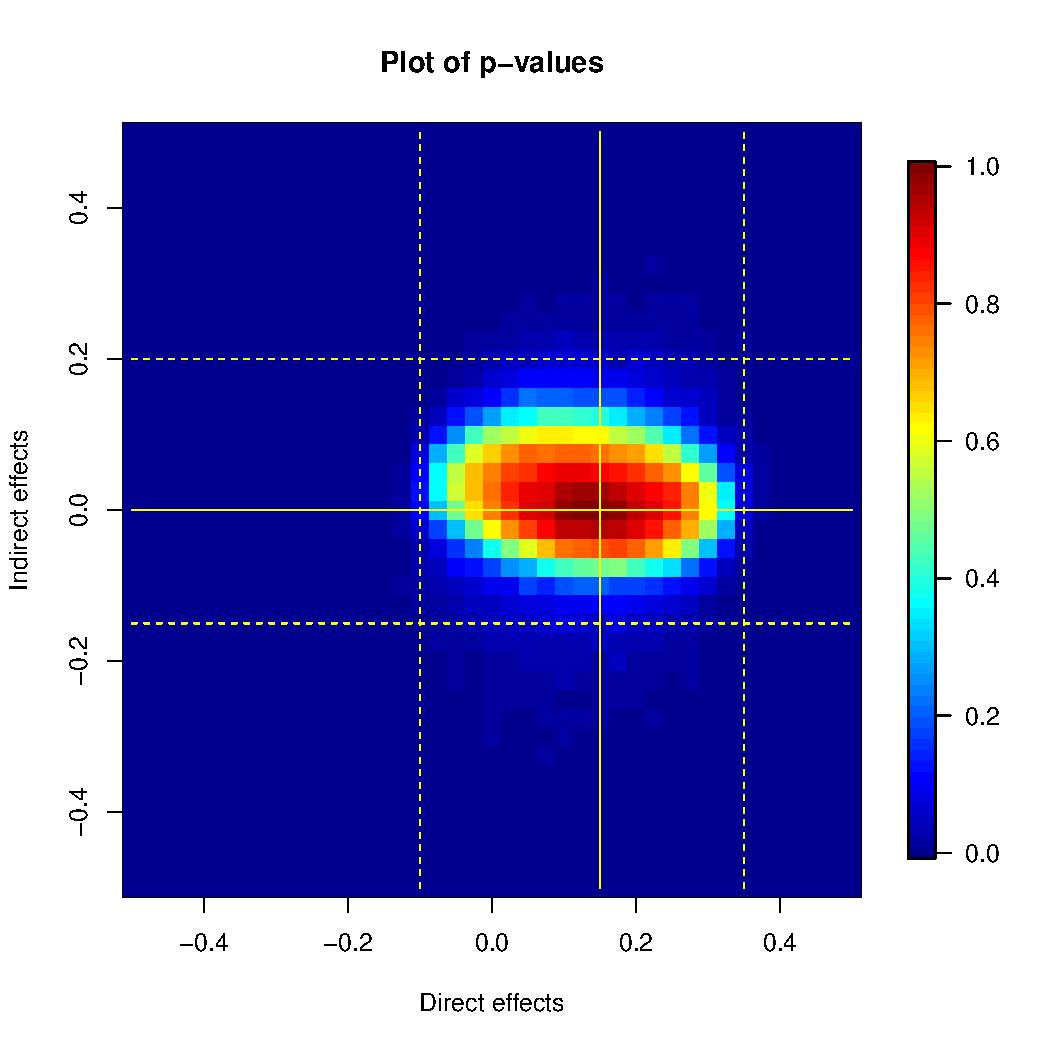
\includegraphics[scale=0.45]{./images/pval_plot_bergan_main.pdf}
	\end{tabular}
	\caption{p-values: main analysis for \citet{bergan2015call} data}
\end{figure}


Figure 5 depicts results of analyzing the \citet{bergan2015call} data under the ideological network and considers k nearest neighbors (k = 3,5,8,12) based on ideological similarity to constitute the neighborhood. We see that the results regarding indirect effects do not change and the estimate is still zero, indicating no interference effect. Since there is no change in the interference effect estimate, we see no change in the direct effect estimate, which indicates a 15 percentage point increase in the likelihood of voting in favor of the bill in response to being assigned to treatment.

\begin{figure}
	\centering
	\begin{tabular}{cc}
	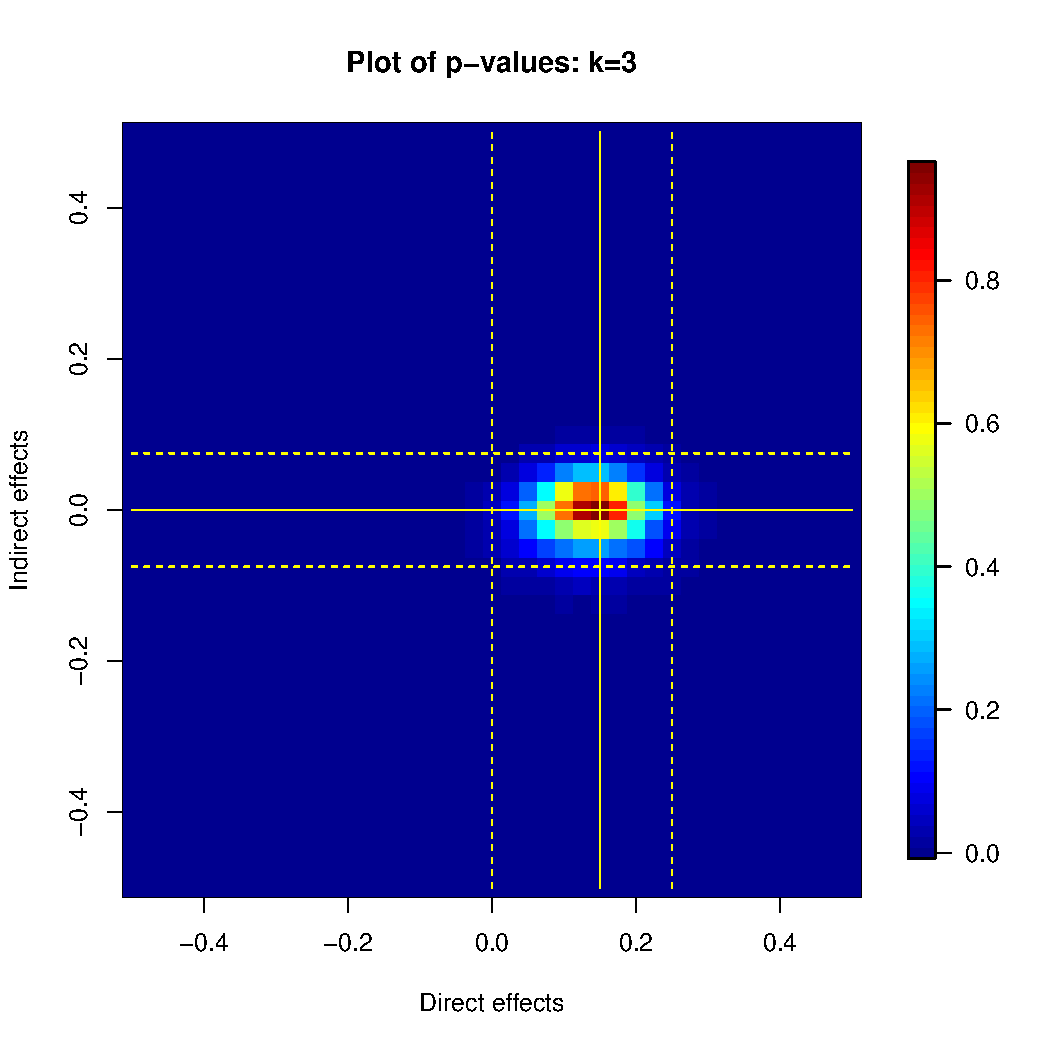
\includegraphics[scale=0.45]{./images/pval_plot_bergan_ideo_3nn.pdf} &
	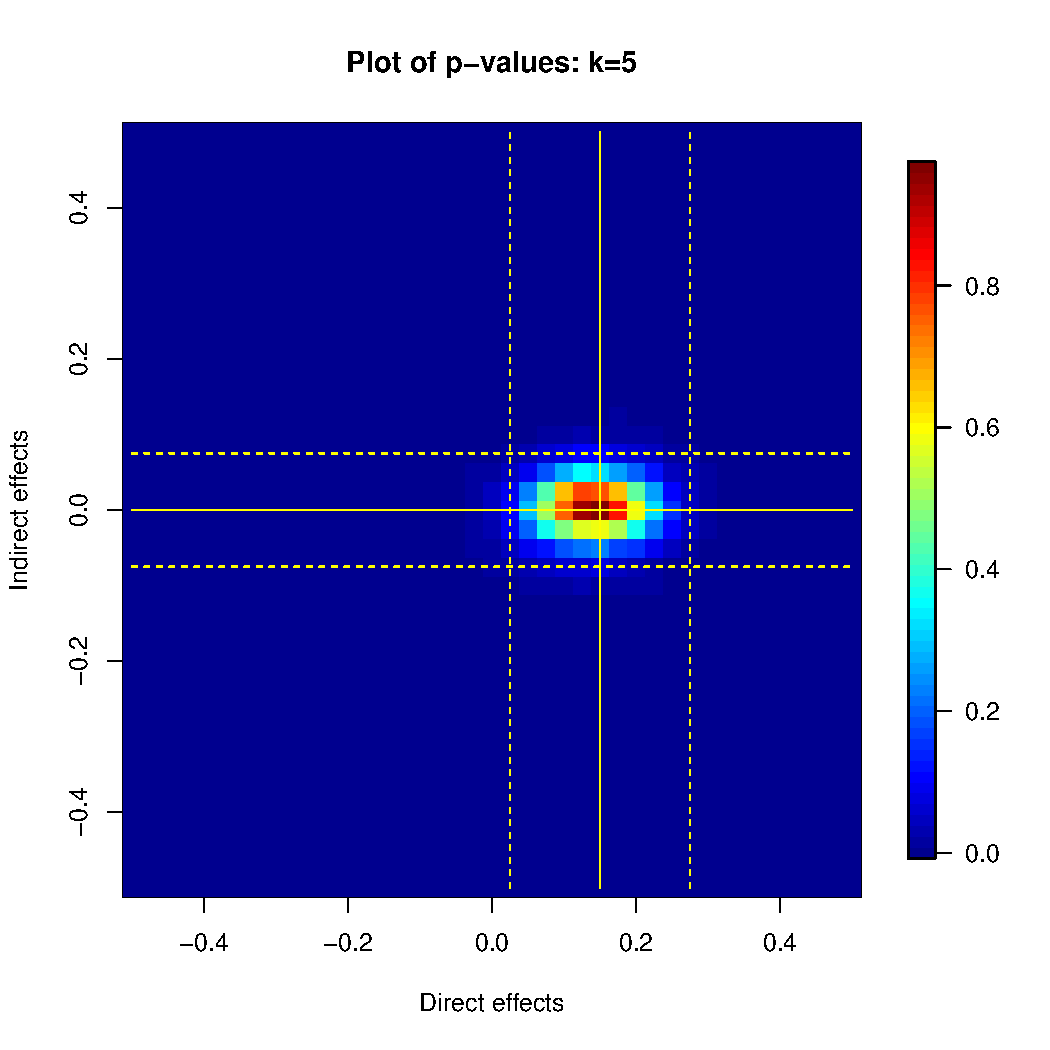
\includegraphics[scale=0.45]{./images/pval_plot_bergan_ideo_5nn.pdf} \\ 
	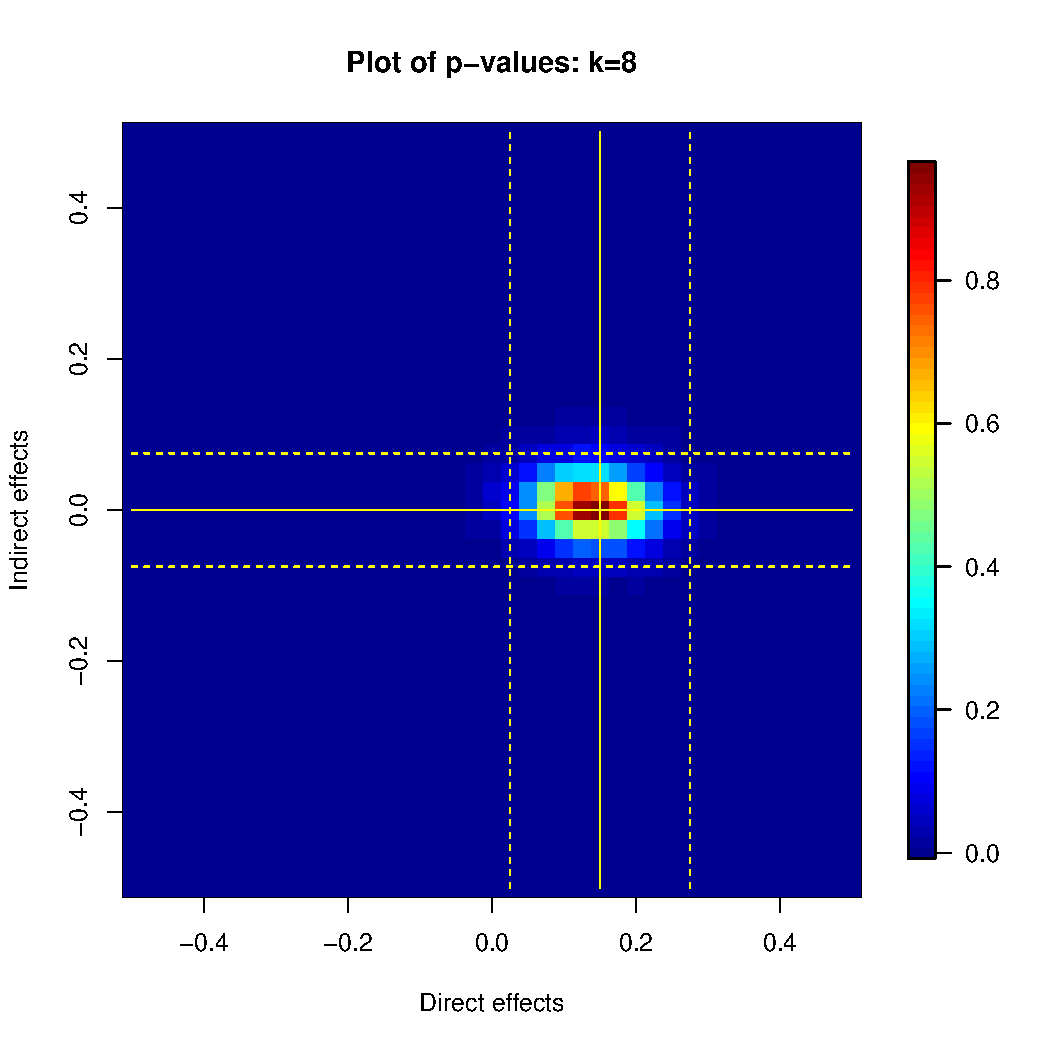
\includegraphics[scale=0.45]{./images/pval_plot_bergan_ideo_8nn.pdf} &
	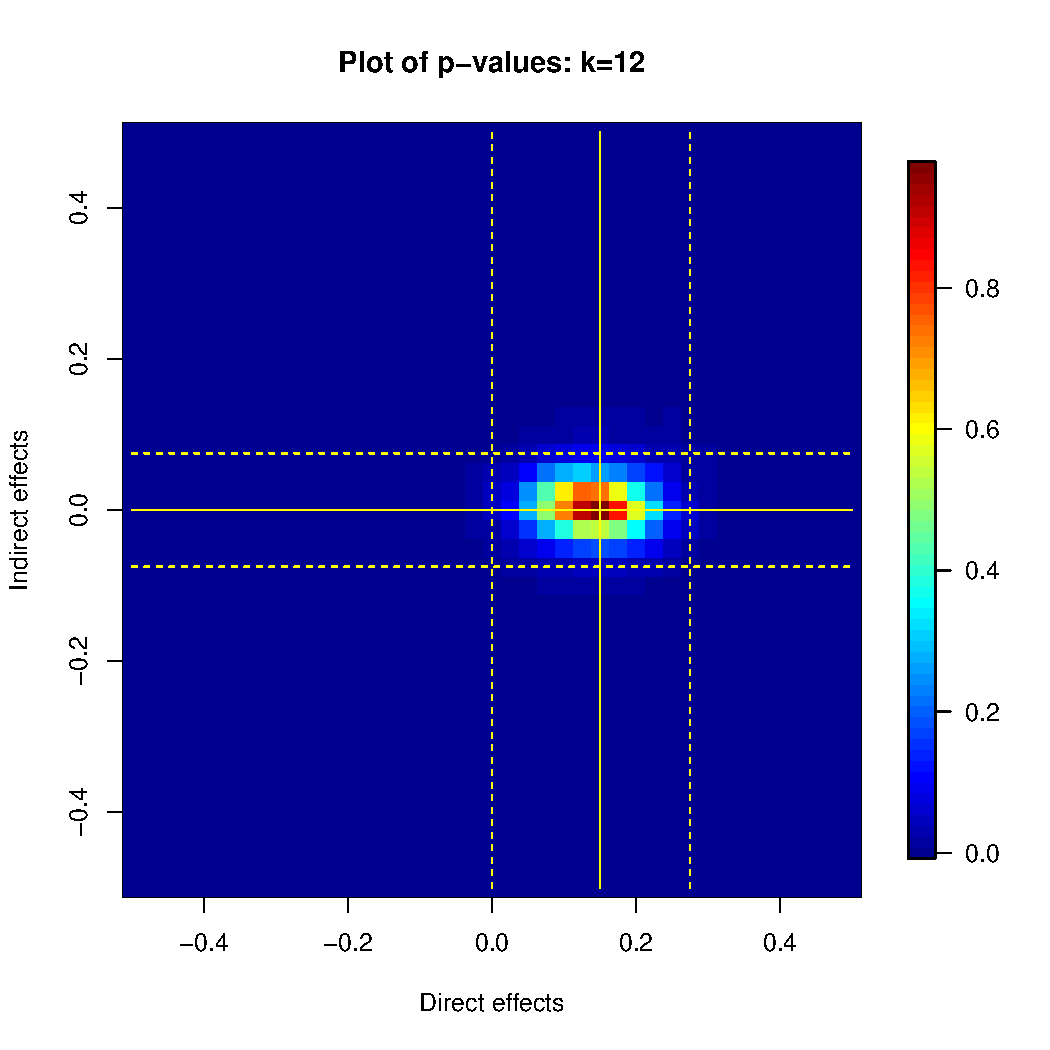
\includegraphics[scale=0.45]{./images/pval_plot_bergan_ideo_12nn.pdf} \\ 
	\end{tabular}
	\caption{p-values: k-nearest ideological neighbors for \citet{bergan2015call} data}
\end{figure}


We again consider an extension in which we change the network. In this network, an undirected edge represents the number of bills cosponsored by a pair of legislators. The indirect effect estimate with this network is positive. The positive indirect effect indicates that as exposure through cosponsorship neighbors goes up, the likelihood of a legislator voting in favor of the anti-bullying bill goes up. However, the confidence interval indicates that this effect is not statistically significant.

\begin{figure}
	\centering
	\begin{tabular}{cc}
	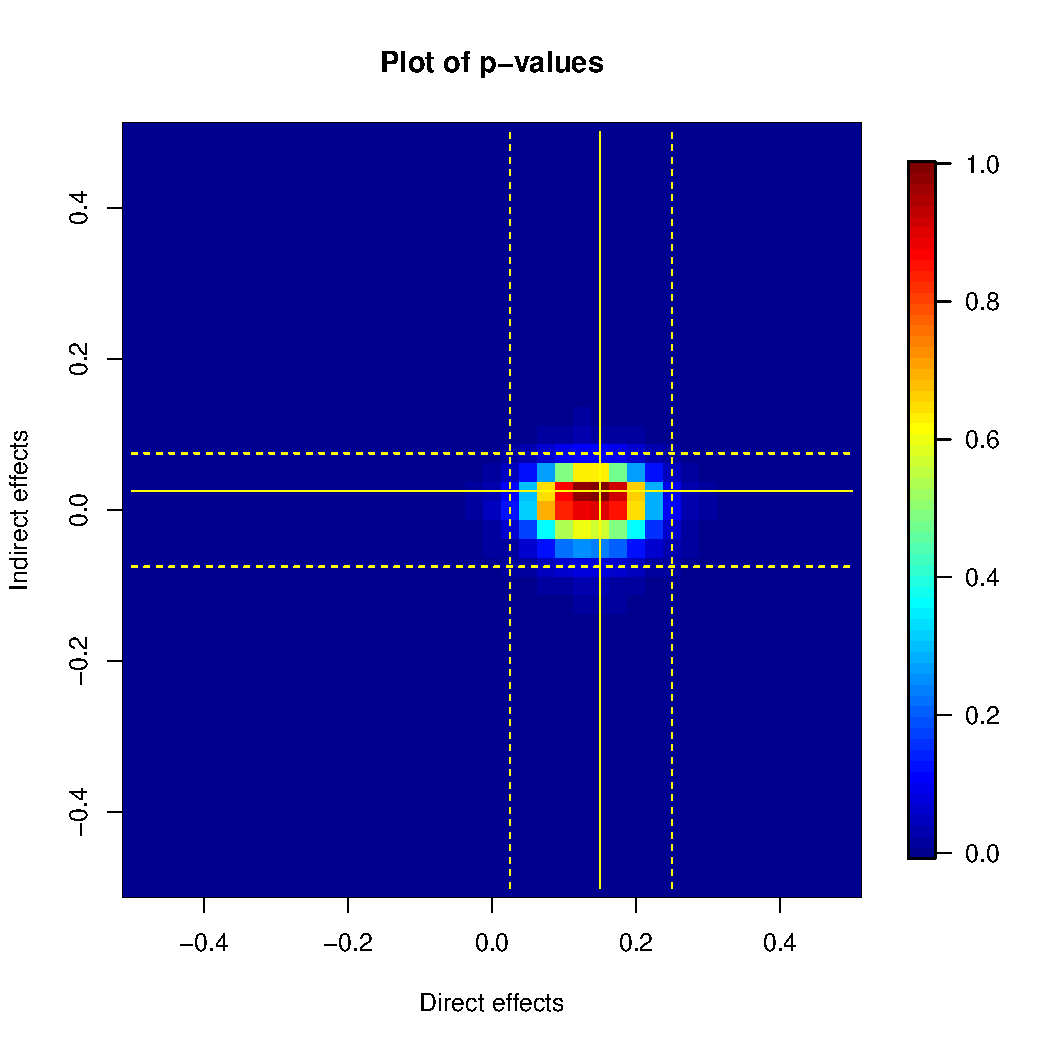
\includegraphics[scale=0.45]{./images/pval_plot_bergan_cospon.pdf}
	\end{tabular}
	\caption{p-values: Cosponsorship network for \citet{bergan2015call} data}
\end{figure}

\floatsetup[table]{objectset=centering,capposition=top}
\begin{table}[h]
\centering
\begin{tabular}{lcccc}
\toprule
\multirow{2}{*}{Model} & \multicolumn{2}{c}{Direct effect} & \multicolumn{2}{c}{Indirect effect} \\
\cmidrule(l){2-3} \cmidrule(l){4-5}
 & Estimate & 95\% CI & Estimate & 95\% CI \\
\midrule
Ideology: full network  & 0.15 & (-0.1, 0.35) &  0 & (-0.15, 0.2)\\
Ideology: 3nn & 0.15 & (0, 0.25) & 0 & (-0.075, 0.075)\\
Ideology: 5nn & 0.15 & (0.025, 0.75) & 0 & (-0.075, 0.075)\\
Ideology: 8nn & 0.15 & (0.025, 0.75) & 0 & (-0.075, 0.075)\\
Ideology: 12nn & 0.15 & (0, 0.275) & 0 & (-0.075, 0.075)\\
Cosponsorship & 0.15 & (0.025, 0.25) & 0.025 & (-0.075, 0.075)\\
\bottomrule
\end{tabular}
\caption{Results from \citet{bergan2015call} data}
\end{table}


%\floatsetup[table]{objectset=centering,capposition=top}
%\begin{table}[h]
%\centering
%\begin{tabular}{lcccc}
%\toprule
%\multirow{2}{*}{Model} & \multicolumn{2}{c}{Direct effect} & \multicolumn{2}{c}{Indirect effect} \\
%\cmidrule(l){2-3} \cmidrule(l){4-5}
% & Estimate & 95\% CI & Estimate & 95\% CI \\
%\midrule
%Ideology: full network  & 0.125 & (0.025, 0.2) &  -0.05 & (-0.45, 0.5)\\
%Ideology: 3nn & 0.1 & (0, 0.2) & -0.05 & (-0.25, 0.05)\\
%Ideology: 5nn & 0.1 & (0, 0.2) & -0.05 & (-0.175, 0.05)\\
%Ideology: 8nn & 0.125 & (0, 0.225) & -0.025 & (-0.1, 0.05)\\
%Ideology: 12nn & 0.125 & (0, 0.225) & 0 & (-0.075, 0.075)\\
%Cosponsorship & 0.125 & (0.025, 0.2) & 0.075 & (-0.5, 0.5)\\
%\bottomrule
%\end{tabular}
%\caption{Results from \citet{bergan2015call} data: Raw exposure}
%\end{table}


%\subsection{Extensions of Coppock analysis}
%We consider several extensions of the Coppock method, applied to both datasets depending on availability of data.
%
%\begin{itemize}
%\item Consider k (=3, 5, 8, 12) neighbors according to ideological scores to form adjacency matrix. A tie between i and j indicates that legislator j is one of the k-nearest neighbors to i. This generates some ties. We will try the following two ways of taking care of the ties:
%
%\begin{enumerate}
%\item Choose, among the ties in the k closest neighbors for i, those nodes for which i is the closest neighbor. To illustrate, if i is equally close to j and h, we ask whether i ranks higher on j's list of closest neighbors. If yes, then we take out h. If no, we keep j and h if i ranks equally on j and h's neighbor list, or kick out j if h ranks i more highly.
%\item Look at the number of nodes for which j is the nearest neighbor and in some way account for the j's influence on that basis
%1. Look at control unit i
%2. Calculate a composite score that indicates the ranking of i for each of its k neighbors
%3. Estimate a parameter to see if change in composite score leads to a change in propensity for changing the outcome
%4. This parameter will be modeled as a non-linear effect
%For example, say k=3 condition. If a control unit is the lowest in the proximity of all of its 3 neighbors, it is less likely to receive a spillover; as compared to if it was in the highest proximity of all three of them (the two extremes). We would have to condition this on the treatment status of its neighbors.
%\end{enumerate}
%
%\item Consider committee network instead of ideological network, where a tie between i and j indicates that they have served on two or more committees together
%\item Use number of shared committees in adjacency matrix
%\item Separate out the high and low support district in original \citet{butler2011can} data and conduct separate analyses. This would explain the direction of the spillover effect much better. Conduct this analysis with ideological network as well as committee network
%\item Include geographical network in both dataset and extend analysis
%\item Consider various spillover models other than the growth curve specification
%\item Consider weighted combinations of different networks to estimate a $\gamma$
%\item Explore the idea of using communities to model spread across the network
%
%\end{itemize}
%%%%
\section{Conclusion}
%%%%


% What we have demonstrated
In this paper we have advocated that scholars who run field experiments on state legislatures consider testing for interference. We provide guidance in specifying these tests using the methods developed by  \citet{bowers2012reasoning}. Specifically, we discuss options for specifying the network(s) through which interference occurs, selecting the neighborhood of legislators who affect the legislator through the network(s), and specifying the functional form according to which the interference effects manifest. We illustrate this approach with two in-depth replications. We do not find universal evidence for interference effects in our replications. Our mixed findings regarding interference effects are attributable to an actual lack of interference in some contexts, a misspecification of the model of effects (which could include using the wrong network(s)), or some combination of both.  Nonetheless, these replications serve to illustrate the variety of choices researchers have to make when testing for interference effects in experiments on state legislatures. 

{\bf [UPDATE THIS PARAGRAPH WITH RESULTS]}
The results from our replication of field experiments on legislatures underscore the importance and complexity of accounting for interference. The replications and extensions of \citet{coppock2014information} and \citet{broockman2013black} demonstrate modest evidence of interference effects, and the inferential consequences of choices in specifying both the network and the neighborhood through which treatment is hypothesized to propagate. We did not see evidence for spillover effects in any of the specifications for \citet{bergan2015call}.  Our replication study is not intended to provide definitive evidence regarding whether or not state legislative field experiments are subject to interference effects. Rather, we illustrate a broad array of network and neighborhood definitions, and provide evidence that some experiments are characterized by interference effects, and some are not. Given that tools are now available for testing interference effects, researchers have little reason to assume SUTVA in legislative field experiments. Indeed, relaxing SUTVA, and using the methods introduced by \citet{bowers2012reasoning}, enables the researcher to explore myriad hypotheses regarding the presence and structure of interdependence in the legislature. In the replication materials for this article, we include an R package that implements functions for carrying out the testing methodology developed by \citet{bowers2012reasoning}.\footnote{Shortly after this article is accepted for publication, this package will be submitted to the CRAN network for public distribution.}

% Implications for future research
Despite providing preliminary evidence that some state legislative field experiments are characterized by interference, one shortcoming of our replication analyses is that the experiments were designed and data collected with a focus on direct effects, assuming SUTVA. We retrospectively constructed networks to use in testing for interference, relaxing SUTVA, which is not ideal since there are likely to be more appropriate networks for each individual application. In future state legislative field experiments, researchers should consider collecting network data that characterizes the patterns of interdependence between legislators that are most relevant to their experiments. Furthermore, in each of the studies we consider, half of the observations were allocated to treatment, and treatment allocation was uniform-at-random (within blocks). This may not be the optimal randomization design if the researcher is interested in testing for and identifying interference effects. In experiments designed for testing interference effects, the optimal proportion assigned to treatment is typically much lower than 50\% \citep{bowers2016models}. Furthermore,  researchers can use the networks through which they think interference occurs to design higher powered experiments that incorporate the network structure \citep{bowers2016models}. The optimal experimental design depends on the structure(s) of the network(s) through which interference is hypothesized as well as the model of effects. In future work, researchers conducting field experiments on state legislatures should take the networks and models of effects into account at the design stage.


%\clearpage
\bibliographystyle{apsr}
\bibliography{interference}

\end{document}
%%%%
\section{Network plots}
%%%%

\begin{figure}
\centering
\begin{tabular}{cc}
{\bf Geographic Network} & {\bf Committee Network (>1 in common)}\\
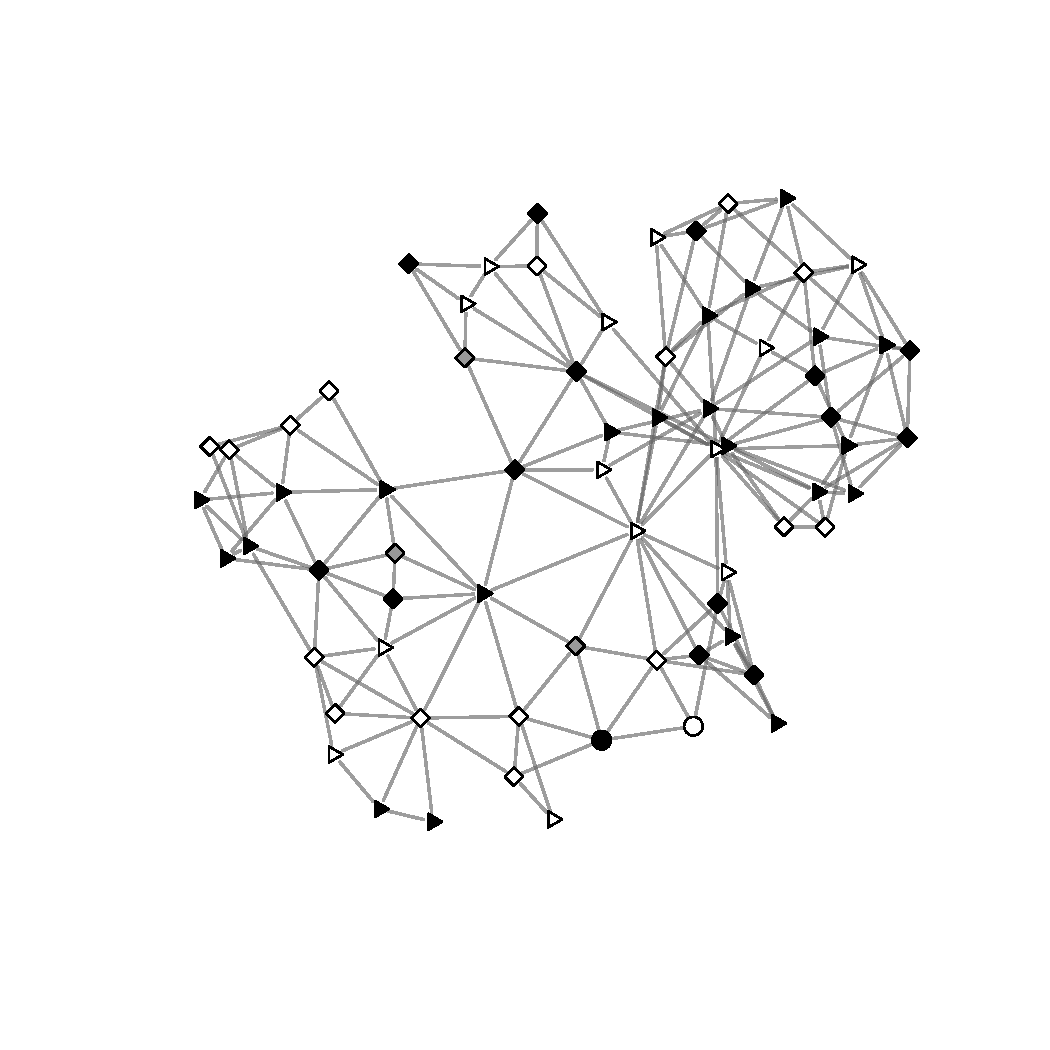
\includegraphics[scale=.55, clip=true,trim =2cm 2cm 2cm 2cm ]{./images/coppock_geographic_net.pdf} & 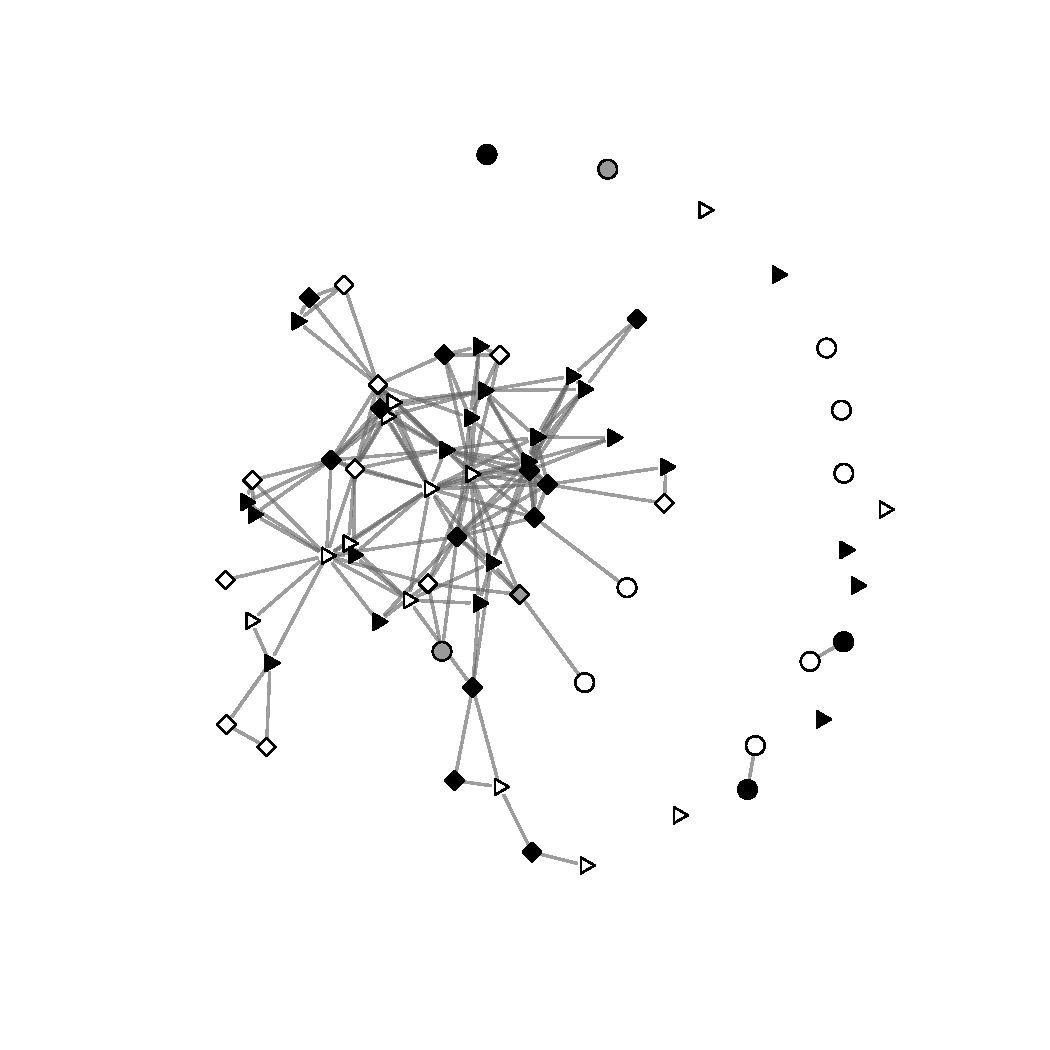
\includegraphics[scale=.55, clip=true,trim =2cm 2cm 2cm 2cm]{./images/nm_committee_net.pdf} \\ 
\end{tabular}
{\bf Ideological Network (top 5\%)} \\
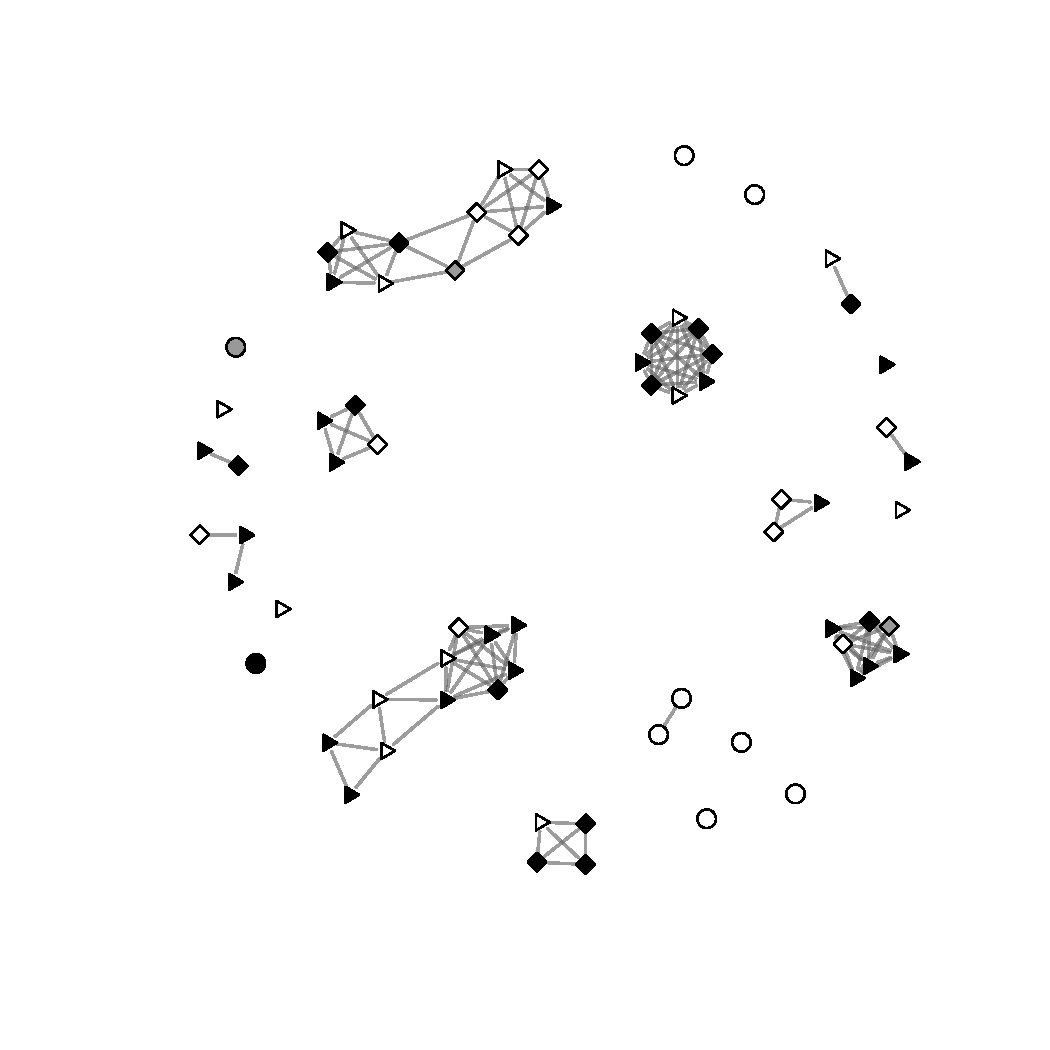
\includegraphics[scale=.55, clip=true,trim =2cm 2cm 2cm 2cm]{./images/coppock_ideological_net.pdf}
\caption{Different networks among New Mexico legislators. Colors denote outcome: black means voted with district, gray means abstained, white means voted against. Shape denotes treatment status. Triangles are treated. Squares are adjacent to treated. Circles are isolated from treatment}
\label{figure: nh-nets}
\end{figure}


%%%%
\section{Appendix}
%%%%

\subsection{Appendix 1A}

In this section, we will look at user-defined R-functions that replicate the \citet{bowers2012reasoning} methodology. This contains four steps:

\begin{itemize}
\item A function to transform the observed outcomes into potential outcomes for any treatment assignment w
\item A function to separate the hypothesized treatment effect
\item A function to calculate test statistic
\item A function to calculate the p-value.
\end{itemize}

The results from the ks.test function in R for calculating Kolmogorov-Smirnoff test statistic are verified with that in Footnote 12 of the paper.


\textbf{Function 1: calculating potential outcomes}

\begin{lstlisting}[language=R]
set.seed(132)

library(doParallel)
library(foreach)
library(kSamples)
library(network)
library(permute)

#### Potential outcomes ####

#### Transform uniformity trial outcome into observed outcome
unif.to.z <- function(z, S, y.0, beta, tau){
  # z: observed treatment assignment
  # S: adjacency matrix
  # y.0: outcome vector for uniformity trial
  # beta: growth curve parameter
  # tau: rate of growth parameter  
  scalar <- as.vector(t(z)%*%S)
  spillover <- rep(NA, n)  
  spillover <- beta + ((1-z) * (1-beta) * exp(-tau^2 * scalar))  
  # This is equation 4
  h.y0.z <- spillover*y.0
}

#### Transform observed outcome into uniformity trial outcome
z.to.unif <- function(z, S, y.z, beta, tau){
  # z: initial treatment assignment
  # S: adjacency matrix
  # y.z: observed outcome vector
  # beta: growth curve parameter
  # tau: rate of growth parameter
  scalar <- as.vector(t(z)%*%S)
  spillover <- rep(NA, n)  
  # Equation (3) from paper
  spillover <- beta + ((1-z) * (1-beta) * exp(-tau^2 * scalar))
  # Equation (5) from paper
  h.yz.0 <- (1/spillover)*y.z
}

#### Transform observed outcome into outcome for ANY other assignment w
z.to.w <- function(z, S, w, y.z, beta, tau){
  # z: initial treatment assignment
  # S: adjacency matrix
  # w: new treatment assignment
  # y.z: vector of outcomes for z
  # beta: growth curve parameter
  # tau: rate of growth parameter
  scalar.z <- as.vector(t(z)%*%S)
  scalar.w <- as.vector(t(w)%*%S)
  
  spillover.z <- rep(NA, n)
  spillover.z <- beta + ((1-z) * (1-beta) * exp(-tau^2 * scalar.z))
  
  spillover.w <- rep(NA, n)
  spillover.w <- beta + ((1-w) * (1-beta) * exp(-tau^2 * scalar.w))
  
  # Equation (6) from paper
  h.z.to.w <- (spillover.w / spillover.z) * y.z
}

#### Testing and p-value calculation ####
p.val <- function(z, y.z){
  
  cl <- makeCluster(4) #Setup for parallel computing
  registerDoParallel(cl)
    
  # Calculate the outcome vector after taking away the effect of treatment
  y.0 <- z.to.unif(z=z, S=S, y.z=y.z, beta=beta, tau=tau)
  
  # Calculate test statistic
  test.stat <- ks.test(y.0[z==1], y.0[z==0],
                       alternative = "g")$statistic
  sign <- noquote(strsplit(names(test.stat), NULL)[[1]])[3]
  if(sign=="+"){
    test.stat <- test.stat
  }else{
    test.stat <- test.stat*-1
  }  
  
  # Calculate a vector of test statistic using permutations
  results <- foreach (i = 1:perms) %dopar%{
    require(permute)
    perm.z <- z[sample(1:length(z),length(z),rep=F)]
    perm.test.stat <- ks.test(y.0[perm.z==1], y.0[perm.z==0],
                              alternative = "g")$statistic
    sign <- noquote(strsplit(names(perm.test.stat), NULL)[[1]])[3]
    
    if(sign=="+"){
      return(perm.test.stat)
    }else{
      return(perm.test.stat*-1)
    }
  }
  stopCluster(cl)
  
  # A vector of test statistics
  all.test.stat.vals <- unlist(results)
  
  # Calculating p-value
  pval <- sum(all.test.stat.vals > test.stat)/perms
  return(pval)
}
\end{lstlisting}


\subsection{Appendix 1B}

Below code replicates the \citet{coppock2014information} results using the framework setup in the Bowers replication code

\begin{lstlisting}[language=R]

set.seed(231)
library(doParallel)
library(fields)
library(foreach)
library(kSamples)
library(network)
library(permute)
library(wnominate)

permute.within.categories <- function(categories,z){
	ucategories <- unique(categories)
	perm.z <- rep(NA,length(z))
	for(c in ucategories){
		z.c <- z[which(categories==c)]
		perm.z.c <- sample(z.c,length(z.c),rep=F)
		perm.z[which(categories==c)] <- perm.z.c
	}
	perm.z
}

#### Read the original Butler and Nickerson data
data <- read.table("nm.replication.tab", sep="\t", header=TRUE)
z <- data$treatment #observed treatment
y.z <- data$sb24 #observed outcome
n <- length(y.z) #number of observations
t <- length(z[z==1]) #number of treated units
perms <- 10000 #number of permutations to use in generating expected exposure
perms.test <- 5000 #number of permutations used in testing

# Function to generate adjacency matrix using similarity scores
get.similarity <- function(x, y){
  return((2-abs(x-y))/2)
}

load("CoppockJEPS.rdata")
dwnom_scores <- CoppockJEPS$dwnom_scores

## Create an adjacency/similarity matrix using ideology
S.ideo <- matrix(NA, ncol=70, nrow=70)
for (i in 1:70){
  for (j in 1:70){
    S.ideo[i,j] <- get.similarity(dwnom_scores[i], dwnom_scores[j])
  }
}
diag(S.ideo) <- 0
S.ideo[is.na(S.ideo)==T] <- 0


#### Generate expected exposure
perm <- replicate(perms, permute.within.categories(data$match_category,z))
expected.exp0 <- rep(0, n)
expected.exp1 <- rep(0, n)
for(p in 1:ncol(perm)){
  zp <- perm[,p]
	for(i in 1:n){
		if (zp[i] == 1){
				expected.exp1[i] <- expected.exp1[i] + sum(S.ideo[i,]*zp)
			}
			else{
				expected.exp0[i] <- expected.exp0[i] + sum(S.ideo[i,]*zp)
			}
	}
}
num_treat <- apply(perm,1,sum)
num_control <- apply(1-perm,1,sum)
expected.exp1 <- expected.exp1/num_treat
expected.exp0 <- expected.exp0/num_control

#### Generate expected and net exposure
#### This is the spillover effect model
indirect.treatment <- function(permutation, adj.mat){ #any treatment assignment vector and adjacency matrix can be used
 # permutation: can be the initial treatment assignment or a permutation
 raw.exp <- rep(NA, n)
 for (i in 1:n){
   raw.exp[i] <- sum(adj.mat[i,]*permutation)
   }
 net.exp <- raw.exp - (permutation*expected.exp1 + (1-permutation)*expected.exp0)
 standard.exp <- (net.exp - mean(net.exp))/sd(net.exp) #this is the spillover or indirect effect
 return(standard.exp)
}

#### We now model the uniformity trial transformation
z.to.unif <- function(outcome, beta1, beta2, permutation, adj.mat){
  # outcome: vector of direct treatment outcomes
  # beta1: direct treatment effect parameter
  # beta2: indirect treatment effect parameter
  # permutation: vector of a permutation of z (can be z itself)
  # adj.mat: adjacency matrix
  exposure <- indirect.treatment(permutation, adj.mat)
  # This is equation 5
  h.yz.0 <- outcome - (beta1*permutation) - (beta2*exposure)
  return(h.yz.0)
}

#### Testing and p-value calculation
beta1s <- seq(from=-0.5, to=0.5, by=.025)
beta2s <- seq(from=-0.5, to=0.5, by=.025)
pvals <- matrix(NA, length(beta1s), length(beta2s))

cl <- makeCluster(8) #Setup for parallel computing
registerDoParallel(cl)
pvalues.ideology <- foreach (i = 1:length(beta1s)) %do% {
  abc <- foreach (j = 1:length(beta2s)) %do% {
    # Calculate observed test statistic
    exposure <- indirect.treatment(permutation = z, adj.mat = S.ideo)
    test.stat <- sum((lm(y.z ~ z + exposure, na.action = na.omit)$resid)^2)
    
    # Calculate a vector of test statistic using permutations
    results <- foreach (k = 1:perms.test) %dopar% {
      require(permute)
      perm.z <- perm[,sample(1:perms, 1)]
      perm.exposure <- indirect.treatment(permutation = perm.z, adj.mat = S.ideo)  
      perm.y.0 <- y.z + (-1 * beta2s[j] * indirect.treatment(permutation = z, adj.mat = S.ideo))
      perm.y.0[z==1] <- perm.y.0[z==1] - beta1s[i]  
      y.sim <- perm.y.0 + beta1s[i]*perm.z + beta2s[j]*perm.exposure
      perm.test.stat <- sum((lm(y.sim ~ perm.z + perm.exposure, na.action = na.omit)$resid)^2)
      }
    # A vector of test statistics
    all.test.stat.vals <- as.numeric(unlist(results))
    # Calculating p-value
    pval <- sum(all.test.stat.vals < test.stat)/perms.test
  }
  as.numeric(unlist(abc))
}
stopCluster(cl)

for (i in 1:length(beta1s)){
  pvals[i,] <- unlist(pvalues.ideology[i])
}

pvals #rows are direct effects, columns indirect

# Saving results
high.p.value <- max(pvals)
highest.p.indices <- which(pvals==max(pvals), arr.ind = TRUE)
direct.effect.PI <- beta1s[which(pvals==max(pvals), arr.ind = TRUE)[1]]
indirect.effect.PI <- beta2s[which(pvals==max(pvals), arr.ind = TRUE)[2]]
direct.effect.CI.high <- beta1s[max(which(pvals[,which(beta2s==indirect.effect.PI)] >= 0.05))]
direct.effect.CI.low <- beta1s[min(which(pvals[,which(beta2s==indirect.effect.PI)] >= 0.05))]
indirect.effect.CI.high <- beta2s[max(which(pvals[which(beta1s==direct.effect.PI),] >= 0.05))]
indirect.effect.CI.low <- beta2s[min(which(pvals[which(beta1s==direct.effect.PI),] >= 0.05))]

## Creating a plot
image.plot(beta1s, beta2s, pvals,
           main = "Plot of p-values",
           xlab = "Direct effects", ylab = "Indirect effects")

# Lines for point estimate
lines(beta1s, rep(indirect.effect.PI, nrow(pvals)),
      type = "l", col = "yellow", lty = 1) #indirect
lines(rep(direct.effect.PI, nrow(pvals)), beta2s,
      type = "l", col = "yellow", lty = 1) #direct

# Lines for 95% CI
lines(beta1s, rep(indirect.effect.CI.low, nrow(pvals)),
      type = "l", col = "yellow", lty = 2) #indirect low
lines(beta1s, rep(indirect.effect.CI.high, nrow(pvals)),
      type = "l", col = "yellow", lty = 2) #indirect high
lines(rep(direct.effect.CI.high, nrow(pvals)), beta2s,
      type = "l", col = "yellow", lty = 2) #direct high
lines(rep(direct.effect.CI.low, nrow(pvals)), beta2s,
      type = "l", col = "yellow", lty = 2) #direct low

\end{lstlisting}


%===================References======================





\end{document}























\subsection{\citet{broockman2013black} }

The final dataset is from a study that aimed to understand whether politicians behave differently based on the expected electoral incentive. The question of whether there exists differential intrinsic motivation to help a constituent based on his or her race is addressed by studying all state legislators in the US serving in mid-November 2010. These 6,928 legislators received an email from an alias---Tyrone Washington---who was seeking help filing for unemployment benefits. Treatment in this case was an indication that Tyrone was from outside the legislator's district. Legislators were block-randomized based on state, party, and race. Analysis of the experiment resulted in an estimate of a 15--30 18.5 percentage point increase in the likelihood of responding to the email when Tyrone was within the legislator's district. The paper also concluded that extrinsic motivation guided response rates from non-black legislators, and the actions of black legislators were less affected by the treatment. We introduce interference effects in the analysis of this experiment by setting up a model similar to the one in \citet{coppock2014information}, where three separate networks are considered.\footnote{We assume that legislators can only be effected by other legislators in the same chamber.}

The Broockman replication presents a tradeoff in terms of the available data. First, the legislators were anonymized in the replication dataset, which means we cannot match them with other legislative data such as ideal point estimates, committee membership, or cosponsorship. On the other hand, the Broockman dataset is by far the largest among our applications---two orders of magnitude larger than our other datasets. We must therefore use what is available in the replication dataset to construct plausible networks among legislators. We stipulate three possible networks through which interference may occur. These depend on two key covariates; Percentage of Democratic vote for president in the district, and Percentage of black population in the district. We create one network for each of the two covariates and a third combining the two. In networks based on individual variables, the similarity score for legislators $i$ and $j$ based on variable $X$ is defined as in Equation (1).

\begin{equation}
Similarity_{(i,j)} = \frac{2 - |x_i - x_j|}{2}
\end{equation}

For the network based on two covariates, the network is defined as the Euclidean distance between legislators $i$ and $j$ where the two variables---$X$ and $Y$---are equally weighted, as shown in Equation (2).

\begin{equation}
Similarity_{(i,j)} = \sqrt{{(x_i - x_j)}^2 + {(y_i - y_j)}^2}
\end{equation}

In these block-diagonal networks, the neighborhood of any legislator consists of all other legislators in his/her state. The closer any two units are on values of one of these variables, the stronger the tie, and higher the exposure to receiving indirect treatment. Figures 6 and 7 depict results of analyzing the \citet{broockman2013black} data under the combined network and the individual networks respectively. We see that two of these three specifications show evidence of spillover effect. The estimate for the percentage black is negative and marginally statistically significant, indicating that legislators further reduce their responsiveness to a constituent outside their district if other legislators from districts similar in racial composition also receive an outside-the-district contact. The direct effect estimates are robust, and follow the original study. The results are further detailed in Table 5.


\begin{figure}
	\centering
	\begin{tabular}{cc}
	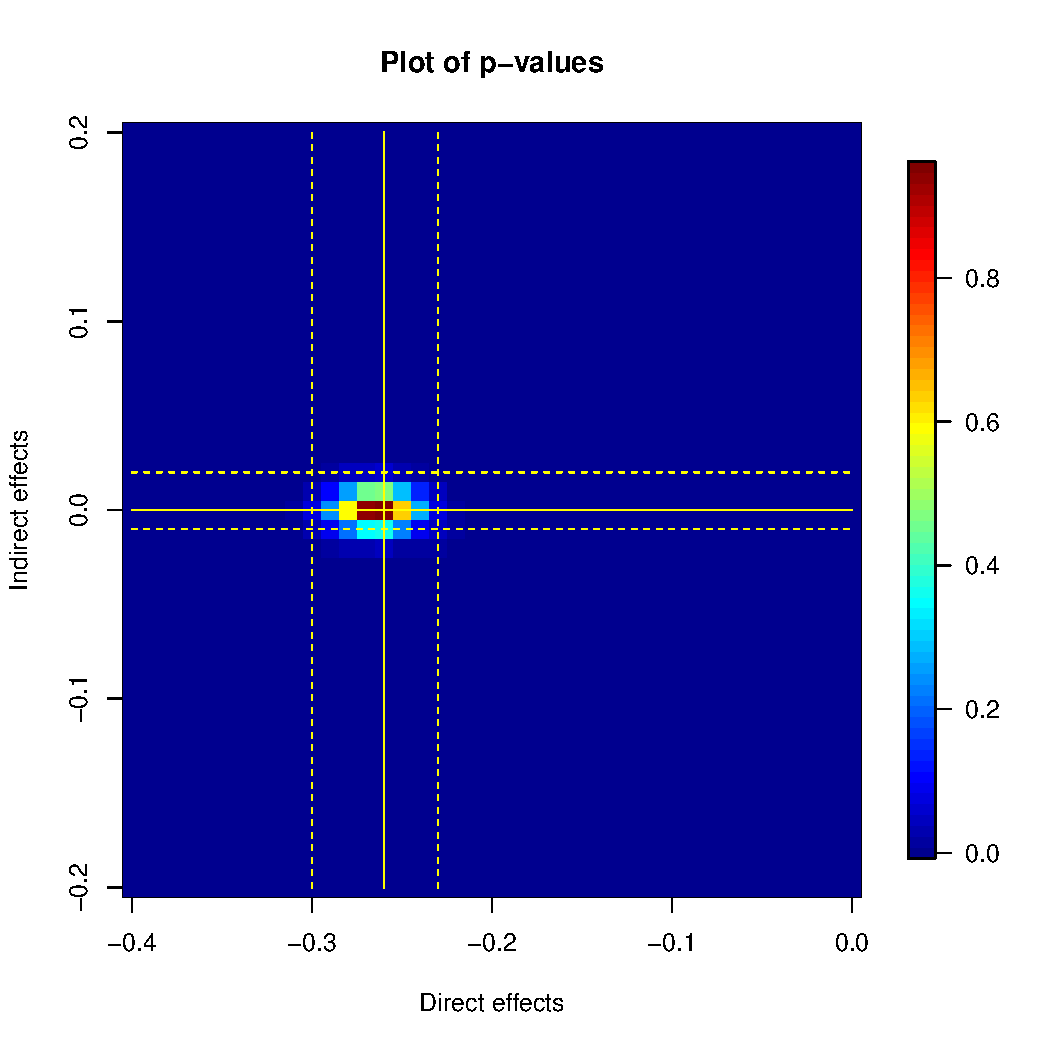
\includegraphics[scale=0.45]{./images/pval_plot_broockman_demvotepct.pdf} &
	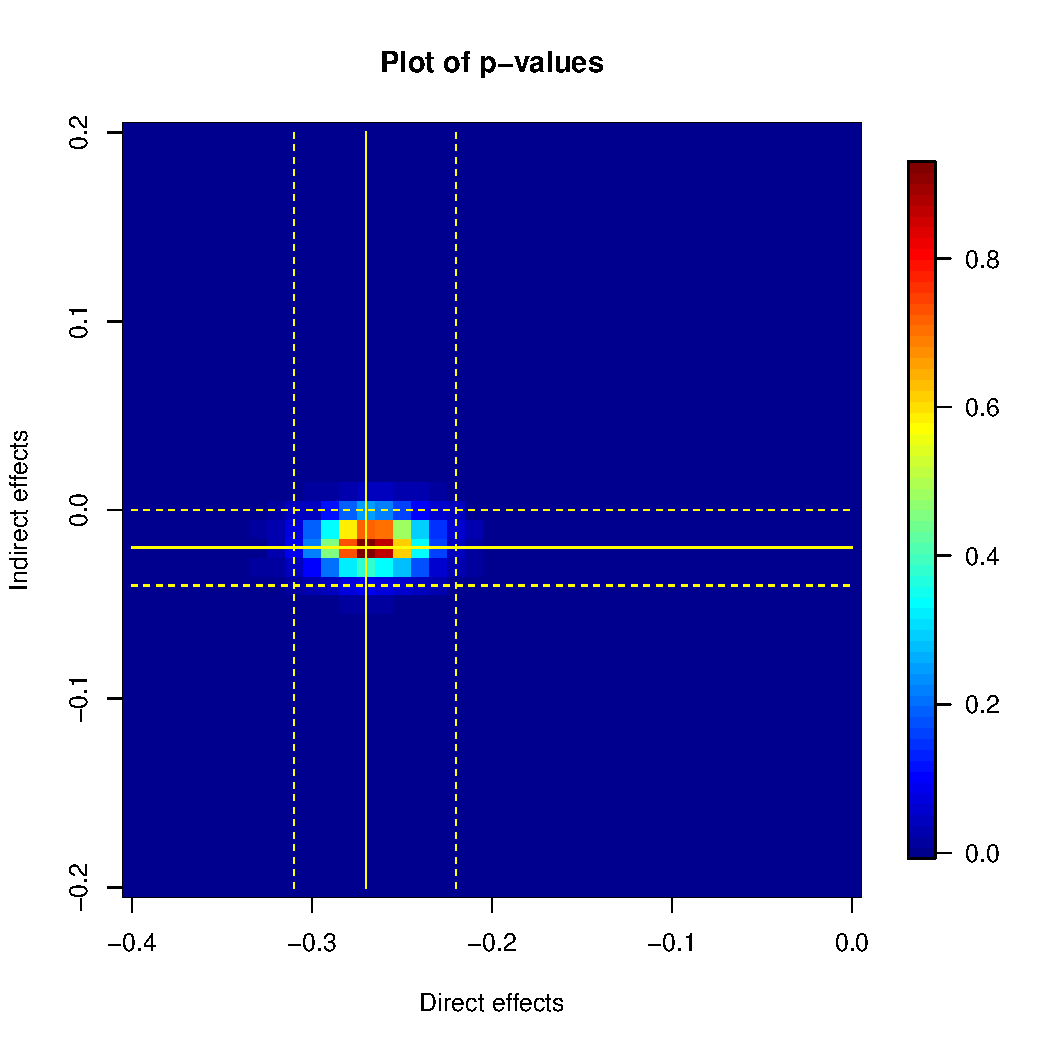
\includegraphics[scale=0.45]{./images/pval_plot_broockman_blackpct.pdf} \\ 
	\end{tabular}
	\caption{p-values for \citet{broockman2013black} data. Percent democratic vote is on the left, and percent black is on the right.}
\end{figure}

\begin{figure}
\centering
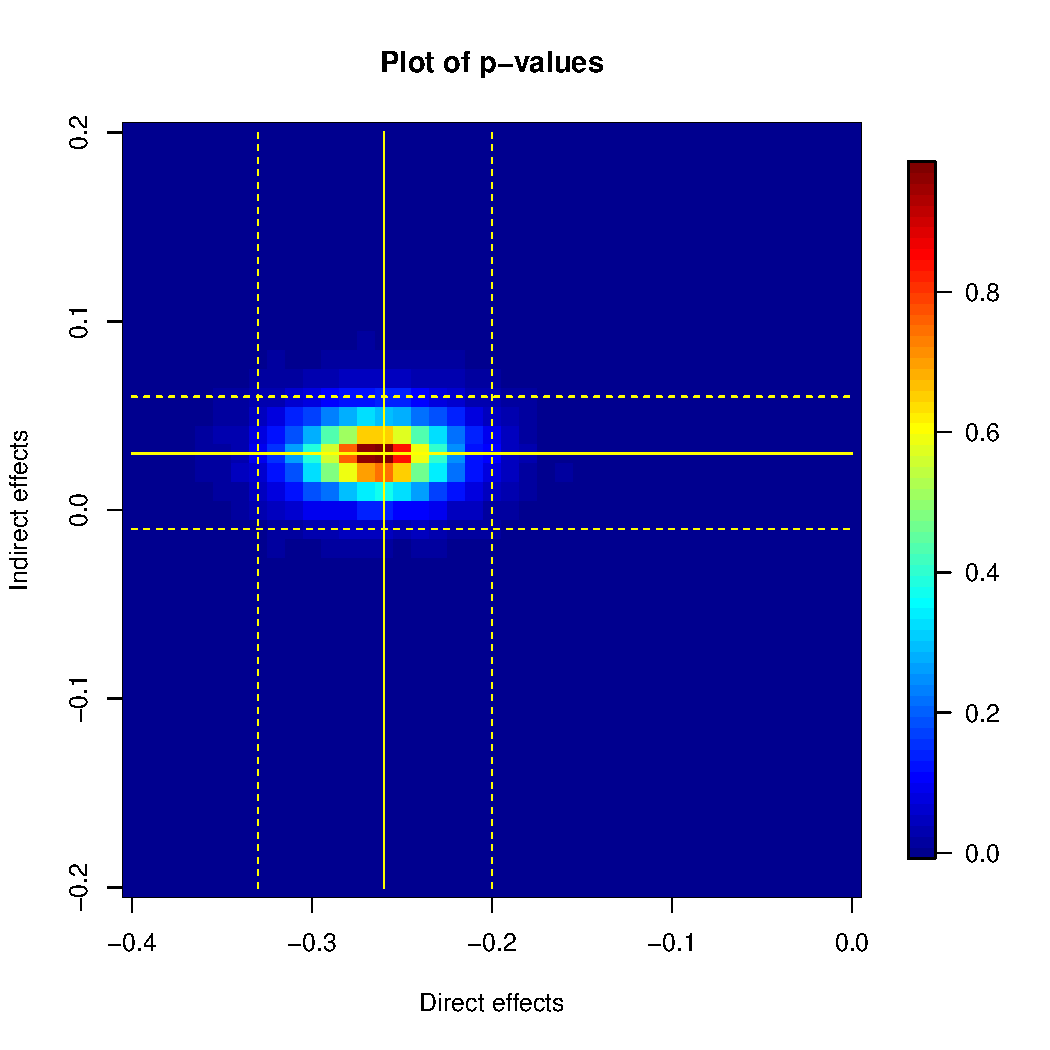
\includegraphics[scale=0.45]{./images/pval_plot_broockman_demvotepct_blackpct.pdf}
\caption{p-values for \citet{broockman2013black} data: Combined network}
\end{figure}



\floatsetup[table]{objectset=centering,capposition=top}
\begin{table}[h]
\centering
\begin{tabular}{lcccc}
\toprule
\multirow{2}{*}{Model} & \multicolumn{2}{c}{Direct effect} & \multicolumn{2}{c}{Indirect effect} \\
\cmidrule(l){2-3} \cmidrule(l){4-5}
 & Estimate & 95\% CI & Estimate & 95\% CI \\
\midrule
Democratic vote percentage & -0.26 & (-0.3, -0.23) &  0 & (-0.01, 0.02)\\
Percentage black & -0.27 & (-0.31, -0.22) &  -0.02 & (-0.04, 0)\\
Mixture network & -0.26 & (-0.33, -0.2) &  0.03 & (-0.01, 0.06)\\
\bottomrule
\end{tabular}
\caption{Results from \citet{broockman2013black} data}
\end{table}


